\documentclass[reprint,aps,prx,superscriptaddress,nofootinbib,longbibliography]{revtex4-2}
\usepackage{eigen-revtex}
\providecommand{\Tr}{\operatorname{Tr}}
\providecommand{\diag}{\operatorname{diag}}
\newcommand{\Ran}{\operatorname{ran}}
\hypersetup{pdftitle={Dynamic Memory},pdfauthor={G. McCaul}}
\begin{document}
\raggedbottom
\title{Dynamic Memory}
\author{G.\ McCaul}
\affiliation{The Laplace Engine}
\begin{abstract}
Memory should make an earlier observation available to a new enquiry, including when its source has changed.
We construct a revisable representation retaining located source contributions beside a joint empirical law.
Prefixes with the same conditional future share a calculation without losing the source identities needed to revise it.
Forward propagation of selected mass and backwards propagation of query tests give the same exact conditional answer.
A worked source correction, addition and retraction exposes the retained dependencies.
On a width-two parity family of 262,144 distinct states, a warm batch of 1024 Boolean queries takes 59.8 microseconds against 1490.7 for packed direct scanning on the tested GPU.
Separate language-delivery studies identify where source conditions and adequate passages help a fixed reader, and where missing observations or temporal composition still prevent recall.
The resulting memory retains a calculation that can be shared, checked against its sources and revised.
\end{abstract}
\maketitle

\section{Memory as a revisable description}
\label{sec:intro}
A memory makes an earlier observation available to a present enquiry.
In a document collection, this means more than preserving the words.
A question may ask which reports concern the same event, how their accounts differ, or what follows when one of them is corrected.
The information needed for recall lies partly in those relations.
We develop Dynamic Memory as a representation that retains them with the source observations on which they depend.

Consider a question comparing two news reports published on different dates.
Finding a paragraph about the right subject is only the beginning.
We need to know which report it belongs to, which date qualifies the statement and what that report actually says.
If the earlier account is corrected, a remembered answer may no longer follow.
The correction must replace its previous contribution rather than masquerade as a second event.
A useful memory needs a route from an answer back to the observations that determine it.

Retrieval-augmented generation supplies a language model with external passages before it answers.
MultiHop-RAG makes the need for several supporting sources explicit~\cite{multihoprag}.
Maximal marginal relevance, or MMR, balances relevance against redundancy in the selected passages~\cite{mmr}.
RAPTOR builds a hierarchy of recursively clustered summaries, offering access at several scales~\cite{raptor}.
These constructions organise access to evidence.
Our question is what calculation a retained representation supports, and what must remain available when its evidence changes.

We begin with a finite joint law of admitted observations - contributions whose fields, weights and source support have been specified.
Each contribution keeps its source revision and a located supporting span.
Observations that have the same conditional future share the remaining calculation, while their source contributions remain distinct.
Sharing equivalent futures is an established way of reducing a predictive description.
Crutchfield and Young reconstruct probabilistic machines by merging equivalent subtrees of observed symbol sequences~\cite{Crutchfield198940eaeb}.
Here equivalence means equality of the remaining empirical distribution at a fixed cut in a finite field order.
The fields need not be successive times, and the corpus need not sample a stationary process.
We therefore use a finite conditional-state quotient, not an inferred stationary \(\epsilon\)-machine or a claim of minimal predictive entropy.

Source-aware calculation also has a precise precedent.
Provenance semirings annotate input tuples and propagate expressions describing how query outputs depend on them~\cite{Green20074d5218}.
Addition records alternative contributions and multiplication records joint use.
A list of contributing sources alone can lose these distinctions.
Our finite construction retains the source-to-tuple incidence beside aggregate prefix counts, then shares equal normalised suffix laws using ordered decision structure~\cite{bryant1986}.
Under fixed field order and admitted positive integer contributions, this combination gives exact conditional answers and an explicit path-copy revision algorithm.
It is not a replacement for general relational provenance or a solution to admitting arbitrary language claims.

There is a separate question about the memory required to realise a stochastic model.
Gu et al.\ encode predictive states as nonorthogonal quantum states and show that quantum models can require less memory than optimal classical models~\cite{Gu2012e2bbbd}.
Our primary calculation is classical.
The operator representation below asks how its selected probabilities embed in a positive channel, not whether a quantum device improves its memory cost.
No quantum memory advantage is measured here.

The construction has two immediate consequences.
A query can be evaluated as propagation through the retained conditional states, in either direction.
A source edit can revise the counts and dependencies that made the answer possible.
We test these consequences with exact finite records and structured query timings.
The language studies test a further interface: whether explicitly conditioned source selection delivers the passages a reader needs.
They do not execute the finite update engine as an end-to-end language system.
An optional extension to a separately specified evolving law is developed in the supporting information.

Figure~\ref{fig:dm-pipeline} sets out these interfaces.
We first establish what a source observation contains, then calculate a recollection and revise its dependencies.
The tests ask where the retained structure saves work and where an answer still fails between available evidence and its use.
A compact representation is useful only after we know what it must preserve.
\begin{figure*}[t]
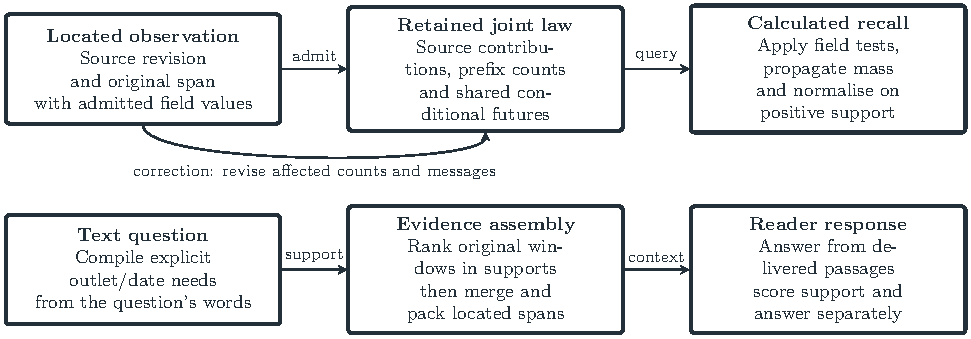
\includegraphics[width=\textwidth]{figures/generated/dm-source-recall-pipeline.pdf}
\caption{From observations to recall.
The upper route is the exact finite construction: admit located observations, retain their joint law, evaluate field tests and revise affected dependencies.
The lower route is the implemented text-delivery study: compile explicit source conditions, rank original passages and supply bounded context to a fixed reader.
Their common interface is identified source support.
Neither the continuous-law extension nor the finite incremental engine is asserted to produce the text answers.}
\label{fig:dm-pipeline}
\end{figure*}

\section{What a source contributes}
\label{sec:object}
The first difficulty is deciding what an observation is evidence for.
A stored extraction from the \emph{Climate} section of the ingested Wikipedia article \emph{Wyoming} describes southeastern tornado vulnerability, a westward decline and tornadoes that tend to be small and brief.
Its located quotation contains only the first claim.
Figure~\ref{fig:dm-wyoming} reproduces the complete three-sentence source unit and the extracted assertion.
It distinguishes the origin of some words from support for the whole assertion.
\begin{figure*}[t]
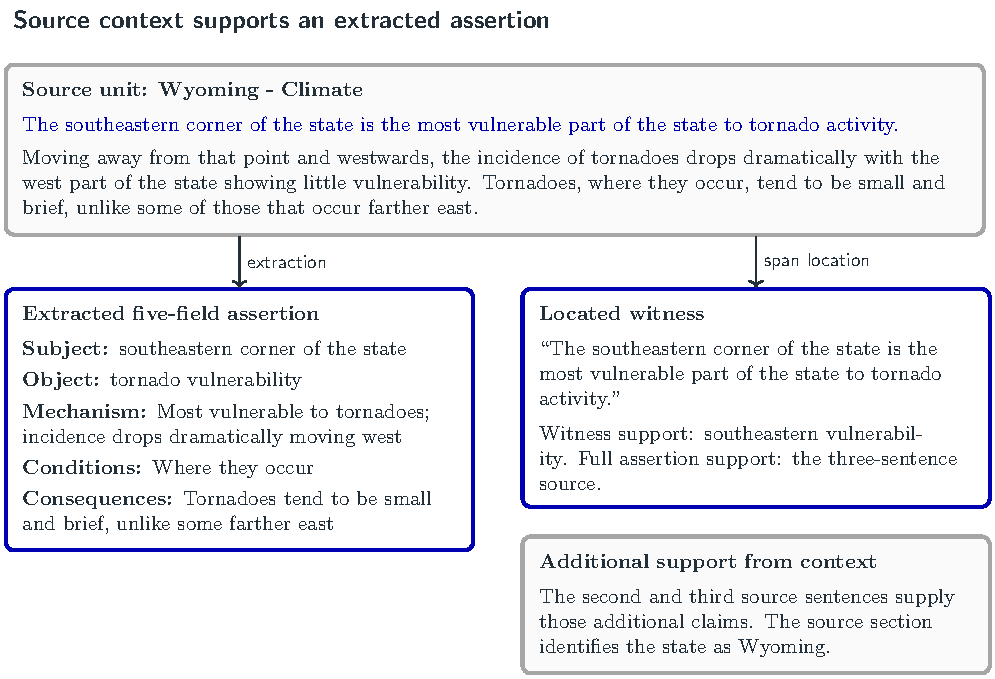
\includegraphics[width=.94\textwidth]{figures/generated/mip_wyoming_witness.pdf}
\caption{A witness must cover the claim it supports.
In the retained Wikipedia plaintext, \emph{Wyoming}, \emph{Climate}, the source unit occupies section-relative characters 1939--2291.
The blue sentence, characters 1939--2037, supports southeastern vulnerability.
The following sentence supplies westward decline, and the last supplies the small, brief character.
The left-hand fields are the stored extraction, not additional source statements.
The example concerns this ingested snapshot, not validation of every extracted field in the corpus.}
\label{fig:dm-wyoming}
\end{figure*}

For an enquiry about duration, the narrow quotation is insufficient.
The implementation nevertheless retains the full five-field \emph{proposal}, the three-sentence input unit and the narrower located quotation.
It does not automatically expand the quotation, split the assertion or reject the additional fields after deciding what they entail.
The proposed consequence remains unsupported by that quotation alone.
Reading the full unit supplies the small-and-brief statement, but this contextual judgement is ours, not an executed entailment gate.

We call a retained source location a \emph{witness}.
The Wyoming record illustrates implemented proposal-and-witness storage, not an admitted weighted row of the calculation below.
Its Subject, Object, Mechanism, Conditions and Consequences are language fields, not the binary \(A,B\) schema used in the controlled example.
No empirical multiplicity for the Wyoming assertion is assigned here.
A source-supported admitted law is an \emph{input condition} of the theory.
If only the narrow span is available, only southeastern vulnerability can be justified from it.
The other proposed claims need broader located support before being used as admitted observations.
Supporting Information~\ref{app:dm-updates} contrasts this condition with the implemented literal parser, where the complete assertion, weight and incidence can all be checked exactly.

Write an admitted observation from source revision \(s\) as a tuple
\(x_s=(x_{s0},\ldots,x_{s,D-1})\) of \(D\) categorical fields, with positive integer multiplicity \(w_s\).
Its joint count, total weight \(W>0\) and empirical probability are
\begin{equation}
 \begin{gathered}
 n(x)=\sum_s w_s\mathbf1[x_s=x],\\
 W=\sum_xn(x),\qquad p(x)=n(x)/W .
 \end{gathered}
 \label{eq:joint-counts}
\end{equation}
The indicator \(\mathbf1[\cdot]\) is one when its condition holds.
Source incidence records which revisions contribute to each tuple.
Distinct batches may contribute to the same tuple.
Repeated reports of one event require an event-identity rule before their weights are added.
Multiplicity is not a confidence score.

Why retain a joint law rather than a separate distribution for each field?
Take equally weighted records \((A,B,C)=000,011,101,110\).
Every field is unbiased and every pair independent.
Nevertheless, among records with \(A=B=0\), the field \(C\) is certainly zero.
The relation survives in the joint records but disappears from their separate marginals.
Tests on fields of one observation must refer to that same joint record and its source contributions.
Combining evidence from several documents will later require an explicit assembly operation, not multiplication of unrelated observations.

A field test is a function \(f_g(x_g)\) between zero and one at ordered position \(g\).
An indicator selects a category, while \(f_g=1\) leaves that field unrestricted.
Their product selects joint evidence.
An unknown value remains an explicit category and does not satisfy a known-value constraint.
The field order is a computational choice.
We now ask how many enquiries can share the work of applying these tests.

\section{Calculating a recollection}
\label{sec:grading}
A small source collection lets us see every step.
Let \(A=0\) select a population and \(B=0\) denote a recorded event.
Two source assertions are
\begin{quote}\small
Group 00 contains 4 records with A=0 and B=0.\\
Group 01 contains 1 records with A=0 and B=1.
\end{quote}
The remaining groups contribute one record at \((A,B)=(1,0)\) and four at \((1,1)\).
All four initial counts are therefore \((4,1,1,4)\).
The selected population contains five records, four reporting the event, giving a recalled fraction \(4/5\).
The literal grammar makes the observation step exact in this controlled example.

Read the fields from left to right.
A \emph{prefix} contains the fields already read.
The remaining fields form a \emph{suffix}, and the boundary between them is a \emph{cut}.
Two supported prefixes share a continuation state when their normalised suffix laws agree.
Table~\ref{tab:dm-states} instantiates the construction for the three-field parity records.
Prefixes \(00\) and \(11\) share the future \(C=0\), while \(01\) and \(10\) share \(C=1\).
Their source records remain individually located.
At cut \(g\), let \(t_g(a,x)\) be the probability of reading category \(x\) from state \(a\), and \(\delta_g(a,x)\) its successor.
\begin{table*}[t]
\caption{Continuation states for equally weighted \(000,011,101,110\), in order \(A,B,C\).
States belong to their labelled cuts, so \(e_1\) and \(e_2\) are distinct.
The terminal has no remaining field and backwards message one.}
\label{tab:dm-states}
\begin{ruledtabular}
\begin{tabular}{clll}
Cut & State: represented prefixes & Remaining law & Next category \(\to\) successor (probability)\\
\hline
0 & root: empty & four tuples, each \(1/4\) & \(A=0\to e_1\;(1/2),\quad A=1\to o_1\;(1/2)\)\\
1 & \(e_1:\;0\) & \(BC=00,11\), each \(1/2\) & \(B=0\to e_2\;(1/2),\quad B=1\to o_2\;(1/2)\)\\
1 & \(o_1:\;1\) & \(BC=01,10\), each \(1/2\) & \(B=0\to o_2\;(1/2),\quad B=1\to e_2\;(1/2)\)\\
2 & \(e_2:\;00,11\) & \(C=0\) & \(C=0\to\mathrm{terminal}\;(1)\)\\
2 & \(o_2:\;01,10\) & \(C=1\) & \(C=1\to\mathrm{terminal}\;(1)\)\\
3 & terminal & empty suffix & stop\\
\end{tabular}
\end{ruledtabular}
\end{table*}

Correct source 00 from four records to three.
The total weight is now nine and \(P(A=0)=4/9\).
For the joint event \(A=0,B=0\), use factor vectors \(f_A=(1,0)\), \(f_B=(1,0)\), in category order \((0,1)\).
For the conditioning event use \(h_A=(1,0)\), \(h_B=(1,1)\).
A backwards message is the probability of passing the \emph{remaining} tests conditional on the current state.
Write \(Z(f)\) for the selected empirical probability mass, before normalising by a conditioning event.
Starting from terminal message one, the event message at \(A=0\) is
\((3/4)\times1+(1/4)\times0=3/4\).
Thus
\begin{equation}
 \begin{gathered}
 Z(f)=\frac49\,\frac34=\frac13,\qquad Z(h)=\frac49,\\
 P(B=0\mid A=0)=\frac{Z(f)}{Z(h)}=\frac34 .
 \end{gathered}
 \label{eq:worked}
\end{equation}
The conditioning query leaves \(B\) unrestricted.
Zero conditioning mass makes the answer undefined, not zero.

The same arithmetic has a linear form.
Let \(S_g\) count continuation states at cut \(g\), and call \(\max_g S_g\) the \emph{continuation width}.
The matrix carrying selected mass to the next cut has \(S_{g+1}\) rows and \(S_g\) columns:
\begin{equation}
 M_g^f[b,a]=\sum_{x:\,\delta_g(a,x)=b}t_g(a,x)f_g(x).
 \label{eq:querymatrix}
\end{equation}
Starting with unit mass \(v_0=1\) at the single root,
\begin{equation}
 \begin{aligned}
 Z(f)&=\mathbf1^{\mathsf T}M_{D-1}^f\cdots M_0^fv_0\\
     &=\sum_xp(x)\prod_{g=0}^{D-1}f_g(x_g).
 \end{aligned}
 \label{eq:querymass}
\end{equation}
The terminal all-ones vector sums surviving mass.
Each path contributes its conditional probabilities, whose product telescopes to \(p(x)\).
This proves the equality and identifies the calculation performed by propagation.

Alternatively, move the test backwards through the transposed matrices.
With terminal message \(m_D=1\),
\begin{equation}
 m_g(a)=\sum_x t_g(a,x)f_g(x)
              m_{g+1}\!\left(\delta_g(a,x)\right).
 \label{eq:adjoint}
\end{equation}
Moving the test backwards in this way is \emph{adjoint evaluation}.
Evaluating the matrix product is often called a \emph{contraction}.
States with equal suffix laws can reuse the same message.
A suffix of unrestricted tests has message one without further work, while a zero branch contributes nothing.
Conditional recall is a ratio of two such calculations under the same law.

The matrix description already answers the classical query.
An operator description adds a different capability: we can ask whether the same selection remains a valid positive operation when this memory is correlated with an auxiliary system.
Represent classical masses \(v(a)\) by the diagonal matrix \(\rho=\diag(v)\).
More generally a \emph{density matrix} is a positive semidefinite matrix, normalised to unit trace for a complete preparation.
Its trace, the sum of its diagonal entries, is total mass.
Off-diagonal entries are called \emph{coherences}.
For each supported pair \((a,x)\), define
\begin{equation}
 K_{g,a,x}=\sqrt{t_g(a,x)f_g(x)}
                |\delta_g(a,x)\rangle\langle a| .
 \label{eq:kraus}
\end{equation}
The ket labels an output state at cut \(g+1\), the bra an input state at cut \(g\).
The sum \(\Phi_g^f(\rho)=\sum_{a,x}K_{g,a,x}\rho K_{g,a,x}^{\dagger}\) is a \emph{Kraus representation}: each operator describes a labelled branch, and summing the branches forgets that label.
It reproduces \(M_g^f\) on diagonal populations and discards coherences.
Its completeness sum is diagonal with entries \(\sum_xt_g(a,x)f_g(x)\leq1\).
Consequently the output trace is surviving mass and cannot exceed the input trace.
Positivity even when an arbitrary auxiliary system is retained is \emph{complete positivity}.
For example, the corrected \(A=0\) state with \(f_B=(1,0)\) sends mass \(3/4\) to the terminal and rejects \(1/4\).
The channel packages this selection as a valid instrument branch.
It does not improve the classical answer or preserve quantum coherence.
Supporting Information~\ref{app:dm-channel} explains the separate square-root amplitude construction.
The field index orders a query calculation, not physical time.

\section{Revising the retained computation}
\label{sec:query}
After the correction, add a distinct batch of one record at \((0,1)\).
The selected counts become \((3,2)\), giving \(3/5\).
Retracting the \emph{old} batch 01 leaves \((3,1)\), giving \(3/4\).
Figure~\ref{fig:updates} follows these operations.
The correction changes the path through \((0,0)\).
Addition and retraction change the path through \((0,1)\).
The \(A=1\) conditional future remains unchanged, although its probability at the root changes.
\begin{figure*}[t]
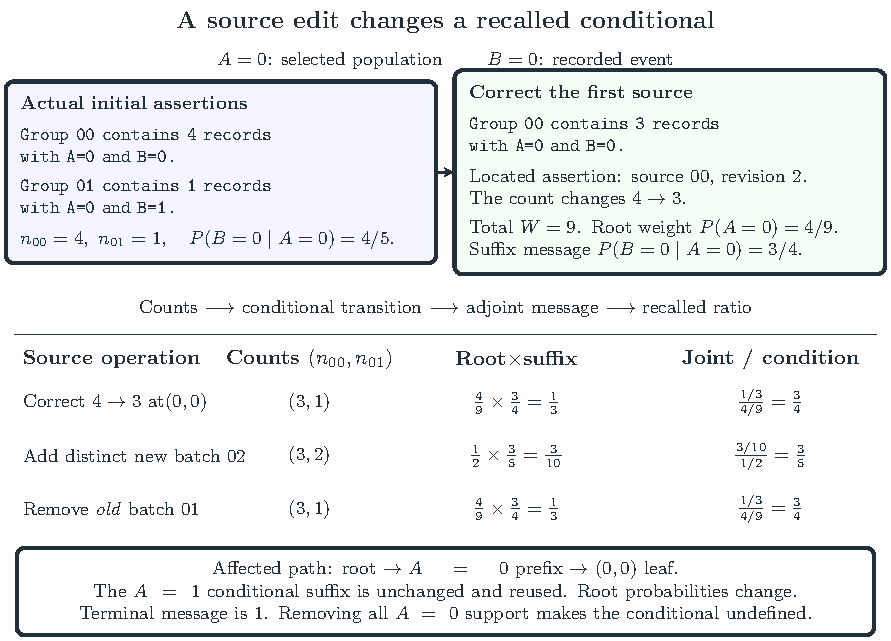
\includegraphics[width=.94\textwidth]{figures/generated/dynamic-memory-witnessed-update.pdf}
\caption{Witnessed source-update calculation, showing the two initial \(A=0\) assertions.
The unchanged \(A=1\) groups have weights one and four.
The bottom path denotes the \((0,0)\) \emph{correction} only.
Addition of batch 02 and retraction of old batch 01 instead use root \(\to A=0\to(0,1)\).
Root mass times suffix message gives the joint event, which is divided by the conditioning mass.
Each operation revises the supported calculation.}
\label{fig:updates}
\end{figure*}

Five stored objects make the update precise.
Source incidence maps an active revision to its tuple contributions and witnesses.
An unmerged prefix occurrence is keyed by its field values, not by a source identity, and holds the aggregate count and child occurrences.
The prefix's canonical signature lists its reduced next-symbol probabilities and successor-signature identities in a fixed order.
Identical signatures share one immutable continuation state.
Reusing states by their signatures is called \emph{hash-consing}.
A query binding associates a raw prefix and query suffix with that state.
The message cache stores a value for a canonical state and those remaining factors.
A binding can become obsolete without making its old cached value false.

For the correction, retract source 00's weight four and add its replacement weight three.
Copy the raw root, \(A=0\) prefix and \((0,0)\) leaf, then rebuild signatures upwards.
The \(A=0\) probabilities change from \((4/5,1/5)\) to \((3/4,1/4)\), so affected bindings must point to the new state.
Messages for the unchanged \(A=1\) signature remain reusable.

Addition of batch 02 makes the distinction between incidence and a prefix explicit.
Sources \texttt{d01-r1} and \texttt{d02-r1} each contribute weight one to the \emph{same} tuple \((0,1)\), with separate assertion witnesses \([0,45)\).
The raw leaf keyed by \((0,1)\) has aggregate count two, not two source-labelled copies.
Its parent \(A=0\) has count five and law \((3/5,2/5)\).
Removing old \texttt{d01-r1} deletes only that incidence entry.
The surviving \texttt{d02-r1} keeps the leaf present with count one.
The parent becomes count four with law \((3/4,1/4)\), so its binding changes.
The old \((3/5,2/5)\) state remains immutable, and both old and new leaves share the terminal's unchanged empty-suffix law.
Supporting Information~\ref{app:dm-updates} gives the actual records and incidence transition.

Raw occurrences are essential when shared futures diverge: counts \((3,1)\) and \((12,4)\) share law \((3/4,1/4)\), but replacing the latter by \((8,4)\) splits them.
Changing their shared state in place would revise the wrong sources.

We can now account for the work by following these dependencies.
Let \(N\) count distinct tuples, \(c_g\) categories at position \(g\), and \(Q\) queries.
If \(A_g\leq Q\) queries remain active after the shortcuts, dense contraction uses
\begin{equation}
 O\!\left(\sum_g A_gS_gc_g\right)
 \label{eq:querycost}
\end{equation}
arithmetic slots, or the visited edges in sparse evaluation.
Direct scanning uses \(O(QND)\) factor work, with packed-word improvements for Boolean tests.
Emitting \(k\) witnesses requires at least \(O(k)\) work.
A single changed tuple touches at most \(D+1\) raw prefix nodes, but source parsing, child-slot copying, rational arithmetic and the affected message cone must also be charged.
A small initial quotient does not guarantee a small update for every change.

Parity explains why continuation size can be more useful than tuple count.
For \(D\) binary fields with even total parity, the \(2^{D-1}\) distinct tuples need only the running parity of the prefix.
Reading one switches parity and reading zero preserves it.
The final field is fixed by the accumulated parity, as in Table~\ref{tab:dm-states}.
This is inherited shared-state structure, not a new parity-complexity result.
The knowledge-compilation perspective is useful because representation size, supported queries and transformations are separate questions~\cite{darwiche2002}.
The tests measure a regime in which the shared conditional calculation is economical.

A different question arises if observations also carry a specified evolution law.
Omitted coordinates may then influence future retained observables even when current retained values agree.
Two preparations can have the same group masses but put different weight on states near an inter-group boundary.
Their later group masses can then differ.
Eliminating that internal imbalance leaves a delayed influence on the retained quantities.
Supporting Information~\ref{app:dm-memory} derives this memory kernel for a finite reversible Markov law, following Mori's projection construction~\cite{mori}.
The saved four-state example there specifies the rates and retained directions and shows what returning omitted information changes.
This optional extension predicts a declared dynamics.
It is neither the source-edit algorithm nor a stage in the language evaluations.

\section{Tests of retained evidence}
\label{section:delivery-under-a-fixed-reader}
The tests address exact conditional calculation, revision of admitted source contributions and delivery of text evidence.
The incremental demonstration is a standard-library CPU implementation.
The structured timing study uses the GPU query implementation, whose source snapshots are rebuilt rather than incrementally revised.
The language studies use separately implemented source-conditioned retrieval.
All text comparisons concern questions already examined during development, including development of the reading instructions.
Within each reported comparison we fix the reader, evidence allowance and endpoint.

\subsection{Exact enquiries}
The edit fixture has nine states and sixteen fixed Boolean product queries.
Forward propagation and backwards messages agree with fresh reconstruction from the active source files and independent direct rational row counts in all 144 query-state checks.
The sequence includes replay, continuation merge and split, and removal of conditioning support.
Supporting Information~\ref{app:dm-updates} gives the assertions, operations and verification costs.
These checks establish the finite implementation outcome, not an incremental scaling advantage.

Figure~\ref{fig:locality} asks whether repeated conditional futures save work when every tuple is distinct.
For even parity, \(D=13,\ldots,19\) gives \(N=4096,\ldots,262144\).
Queries fix selected coordinates and sum over the rest.
The validated integer implementation avoids fractional messages for these Boolean queries (Supporting Information~\ref{app:dm-integer}).
At the largest size, the median over nontrivial tested regimes is \(59.8\,\mu\mathrm{s}\) per warm batch of 1024 queries, against \(1490.7\,\mu\mathrm{s}\) for packed direct scanning.
For one query the values are \(37.4\) and \(45.8\,\mu\mathrm{s}\).
Construction and first compilation are outside these intervals.
The advantage requires reusable conditional structure and enough queries to amortise preparation.
A repeated 64-world support instead favours weighted direct evaluation.
High-entropy unique support reaches width 25,945 and is refused by the continuation kernel's capacity 128.
Supporting Information~\ref{app:dm-timings} gives construction, crossover accounting and these adverse regimes.
\begin{figure*}[t]
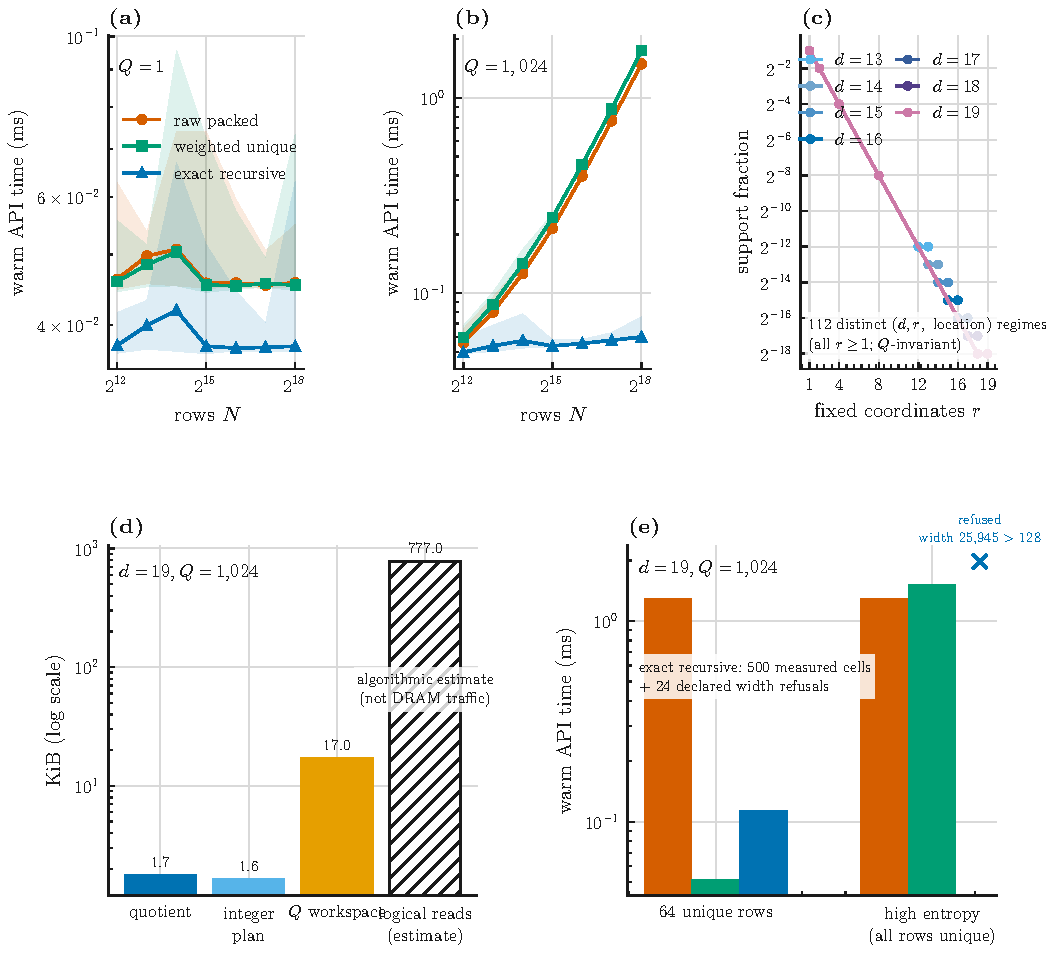
\includegraphics[width=.82\textwidth,viewport=0 246 320 458,clip]{../../../extension/figures/query_locality_completed_v1.pdf}
\caption{Warm full-API latency on the even-parity family.
Only the latency panels are shown: (a) one query, (b) 1024 queries.
Points are medians of per-regime median timings, and shading spans the minimum to maximum across fixed-coordinate counts and locations.
Each regime has two warmups and eleven synchronised samples.
Direct methods scan packed rows or weighted unique rows, which have equal support size here.
The blue curve, labelled \lq\lq exact recursive\rq\rq\ in the saved plot, evaluates continuations by backwards integer messages, with width two.
These are observations on the recorded 4 GB GPU, not hardware-independent latencies.
The complete diagnostic figure and protocol appear in Supporting Information~\ref{app:dm-timings}.}
\label{fig:locality}
\end{figure*}

\subsection{From a question to delivered passages}
For text, an enquiry first becomes explicit requirements and admissible sources.
A deterministic finite grammar recognises outlet names and dates in the news question.
A \emph{facet} is a question-side clause with its recognised bindings.
Here source means the article's outlet, while document identity names a particular article.
Publication dates select exact days.
Event dates or dates of unresolved role use a declared seven-day window, and a named month without a day selects that month.
Unbound axes remain unrestricted.
The compiler reads the question and stored metadata vocabulary, not the answer.
Requirements are supplied identically to all arms in the requirement-table condition.

One actual question asks whether Inter Miami's postseason prospects changed between a Sporting News ticket-price report published on 4 October 2023 and its playoff-exclusion report on 7 October.
The first support set includes both the named ticket report and a separate match report from that outlet on 4 October.
The second includes the 7 October article.
Exact metadata support is therefore not yet exact semantic support.
Within each set, labelled two-sentence windows are scored by cosine similarity of their text vectors plus \(0.5\) times normalised BM25, a keyword relevance score.
The facet-conditioned route takes the next window from each ranked facet in turn, removes duplicates and merges admitted spans in article order.
Its retained 1989-token context discusses rising ticket prices, says Messi did not arrive for the earlier match, and explicitly states later playoff elimination.
The first two observations do not themselves state the earlier postseason assessment.
Supporting Information~\ref{app:dm-text} reproduces this trace and the requirement-table operation.
The example locates missing support rather than inferring an answer from an article title.

The comparison uses 609 articles and 172 MultiHop-RAG questions~\cite{multihoprag}.
All methods receive title/outlet/date-labelled two-sentence windows and 2000 evidence tokens.
The diversity-ranked route applies MMR with relevance coefficient \(0.7\) to 200 candidates.
The local recursive-summary route searches 1747 stored summary nodes plus the labelled windows, without MMR.
It adapts collapsed-tree retrieval by changing leaves and delivery, rather than freshly reproducing public RAPTOR.
The facet-conditioned route may also deliver an explicitly derived support table when it fits within one quarter of the allowance.
This table is not an original passage.
No statement-field score or query-time diffusion is used here.

\begin{table}[t]
\caption{News answers under common requirement-table reading.
Normalised exact match, Claude Sonnet 5.5 at low effort, 2000 \texttt{cl100k\_base} evidence tokens.
Every method receives the same question requirements and answer schema.}
\label{tab:news}
\begin{ruledtabular}
\begin{tabular}{lr}
Evidence assembly & Exact matches /172\\
\hline
Facet-conditioned &153\\
Diversity-ranked &145\\
Local recursive-summary &147\\
\end{tabular}
\end{ruledtabular}
\end{table}
The instruction asks the reader to identify supporting passage IDs and state what they say for each requirement before answering.
It gives 153 exact matches for facet-conditioned retrieval, against 145 and 147 for the controls (Table~\ref{tab:news}).
Paired discordances are nine wins to one loss and seven to one.
The contexts cover 234, 211 and 205 annotated needed facts respectively.
Coverage means that a located occurrence of a reference fact lies wholly within delivered original spans of its article.
It is not a count of generated statements or a substitute for correctness.

Changing the reader instruction changes the comparison.
With common answer-form rules but no requirement table, the same configurations give 152, 152 and 148 exact matches.
The facet-conditioned route therefore ties diversity ranking under that condition.
The advantage in Table~\ref{tab:news} belongs to a particular assembly-and-reader configuration.
The additional delivered facts show what reaches the reader, but their counts alone do not causally explain the answer difference.
Supporting Information~\ref{app:dm-extra-text} displays this alternate reading in the matched-news figure.

FRAMES tests a related delivery problem~\cite{frames}.
The source-conditioned route starts from fifty ranked pieces, adds evidence from one recovered title-link hop and delivers merged sections within 8000 tokens.
If the reader identifies a missing need, one further retrieval supplies up to 4000 tokens of new spans.
The diversity control has the same allowance.
On 190 questions, the completed comparison gives 127 versus 126 judged correct answers, with seven paired wins and six losses.
A separate lexical containment proxy gives 123 versus 117.
Some ingested Wikipedia pages lack the table rows needed for an answer.
Another retrieval can recover an omitted passage, but not an observation absent from the source bank.
The supporting information specifies the cohort, title matching, judging rubric and exact lexical rule and displays both endpoints.
This comparison measures a configuration-specific delivery outcome, not a general language-memory advantage.

The completed LongMemEval-S comparison~\cite{longmem} exposes a different missing operation.
The two stored arm names \texttt{ours\_keys} and \texttt{dense\_keys} execute the \emph{same} dense score call on the shared index, followed by the same ordering and whole-turn packer.
We call them the shared-dense arms here, rather than implying that one performed a compressed conditional reconstruction.
Both give 44 correct answers at 4000 tokens and 45 at 8000, out of 48 including six abstentions.
Both deliver all annotated turns on 41 of 42 cases with positive evidence, excluding the six abstention questions.
The remaining miss asks for elapsed months since two charity events on consecutive days.
Required primary turns rank 73--134, beyond packing frontiers at ranks 27 and 54.
A paraphrase of one event is present, but the decisive pair is not delivered together.
Supporting Information~\ref{app:dm-extra-text} gives the LongMem figure and hybrid comparison.
The case motivates temporal witness composition before packing, rather than assuming a longer undirected context will suffice.

\section{What a dynamic memory makes possible}
\label{sec:outlook}
Dynamic Memory retains a source-supported calculation.
Joint observations determine conditional transitions, query tests propagate through them, and source incidence identifies what must change after a revision.
Sharing equal futures saves repeated work without making their contributing sources interchangeable.
The worked example demonstrates this advantage where every contribution and answer can be inspected.

Scaling depends on retained structure.
Small continuation width can make many enquiries inexpensive even when all tuples differ.
Construction, witness output and large affected dependency cones remain costs.
The GPU study measures the query benefit in one structured regime, while the CPU demonstration establishes a separate finite update route.
For text, the results show why source conditions, delivered context and reader operation must be considered together.

The next improvements follow from specific missing observations.
Table-aware ingestion should retain row labels and column headers with their values, then test whether the needed relation reaches the same reader.
Temporal retrieval should construct event-pair candidates before ordinary packing and test whether the required dates are jointly delivered.
Larger controlled source changes should measure affected count and message cones alongside parsing, retained history and verification.
These tests ask what a representation makes possible, rather than merely whether a longer context changes a score.

An answer need not be permanent to be a successful recollection.
It must be possible to recover why it followed, and what changed when it stopped following.
That is the practical purpose of retaining the calculation with its evidence.
\clearpage
\appendix
\section{Exact finite construction}
\label{app:dm-conditional}
Fix \(D\) finite categorical fields and a nonempty admitted corpus with positive integer source weights.
For a supported prefix \(u\), let \(n(u)\) be the total weight of all tuples beginning with \(u\).
Its normalised suffix law is \(p(v\mid u)=n(uv)/n(u)\).
At each cut identify exactly those prefixes with equal suffix laws.
Equality gives the same next-symbol probabilities.
Conditioning on a supported next symbol then gives equal remaining laws, so the successor state is well defined.
Unsupported symbols have probability zero and contribute no branch.

Along a supported tuple, successive conditionals telescope:
\begin{equation}
 \begin{aligned}
 \prod_{g=0}^{D-1}t_g(a_g,x_g)
 &=\prod_{g=0}^{D-1}\frac{n(x_0\cdots x_g)}{n(x_0\cdots x_{g-1})}\\
 &=\frac{n(x)}{W}.
 \end{aligned}
\end{equation}
The empty-prefix count is \(W\).
Multiplication by \(\prod_gf_g(x_g)\) and summation over paths proves Eq.~\eqref{eq:querymass}.
Summing paths from the terminal proves Eq.~\eqref{eq:adjoint}.
A suffix of identity tests has conditional probability one.
For an event test \(f\) contained in a conditioning test \(h\), the normalised answer is \(Z(f)/Z(h)\) only when \(Z(h)>0\).
The two calculations must use the same empirical law and source revision selection.

The fixed field order is part of the representation.
The quotient may approach the full prefix trie for a poorly structured law.
Neither conditional sharing nor a citation to ordered decision graphs implies a small representation for arbitrary data.
Likewise, retaining source witnesses does not make witness enumeration free.
The source-to-tuple incidence and unmerged prefix counts are additional stored information, not silently included in the quotient's byte count.

\subsection{Integer messages}
\label{app:dm-integer}
Probability messages can be evaluated without fractions in the validated Boolean setting.
For each continuation node \(a\), write its positive suffix probabilities as primitive integer weights \(c_i/T_a\), where the \(c_i\) have greatest common divisor one and sum to \(T_a\).
Define the scaled message
\begin{equation}
 \widetilde m_a=T_a m_a .
\end{equation}
For a Boolean product test, \(\widetilde m_a\) is the integer sum of the primitive weights that pass the remaining tests.
Thus \(0\leq\widetilde m_a\leq T_a\).
At the terminal, \(T_{\rm term}=1\) and \(\widetilde m_{\rm term}=1\).
For the suffix law \((3/4,1/4)\), the primitive total is four.
The test selecting the first category has scaled message three and probability message \(3/4\).
This conversion is what the integer implementation preserves.

Suppose edge \(a\to b\) has reduced probability \(r/\ell\), with \(\gcd(r,\ell)=1\), and the child's suffix probabilities are \(c_i/T_b\).
The branch weights are \(rc_i/(\ell T_b)\).
Their least common denominator is
\begin{equation}
 \frac{\ell T_b}{\gcd(r,T_b)}.
 \label{eq:dm-branchdenom}
\end{equation}
Taking the least common multiple over supported branches gives the parent's primitive total \(T_a\).
The integer edge multiplier is
\begin{equation}
 J_{a,x}=\frac{T_a\,t_g(a,x)}{T_{\delta_g(a,x)}} ,
\end{equation}
and
\begin{equation}
 \widetilde m_a=\sum_xJ_{a,x}f_g(x)\widetilde m_{\delta_g(a,x)} .
 \label{eq:dm-integer}
\end{equation}
The empirical root count is \((W/T_{\rm root})\widetilde m_{\rm root}\).
We use \(D\) for the number of fields, \(\ell\) for a rational denominator, \(s\) for a source and \(a\) for a continuation node.
Divisibility and overflow checks precede integer execution.
Ordinary float32 or float64 contraction of rational transitions is a separate numerical path.
Signed, non-Boolean or unbounded effects are not automatically integer queries.

\section{Witnessed source revisions}
\label{app:dm-updates}
The initial immutable files contain these exact ASCII assertions, each followed by a newline:
\begin{quote}\small
Group 00 contains 4 records with A=0 and B=0.\\
Group 01 contains 1 records with A=0 and B=1.\\
Group 10 contains 1 records with A=1 and B=0.\\
Group 11 contains 4 records with A=1 and B=1.
\end{quote}
The factor order is \(A,B\), with cardinalities \(2,2\).
Each group denotes a distinct batch.
The parser requires its group identity to match the logical source identity.
For \texttt{d01-r1}, the retained assertion is the complete second line, its weight is one and its tuple is \((A,B)=(0,1)\).
The parser checks the immutable bytes against their supplied hash, the full literal grammar, positive integer weight and group-to-source identity.
It records the whole assertion span and the count's subspan.
A malformed assertion or mismatched group is refused, and the engine checks the total-weight bound before mutation.
Replay of the same revision reads and hashes the bytes but neither reparses nor adds the weight again.
These are implemented admission rules for this literal fixture.
They do not decide whether two natural-language reports describe the same event.
That identity policy, and support for every admitted field, remain required inputs outside this grammar.

The correction changes source 00's count from four to three in a new immutable revision.
Both assertion spans are \([0,45)\), and the count span is \([18,19)\).
The added source says exactly
\lq\lq Group 02 contains 1 records with A=0 and B=1.\rq\rq\
The grammar's \lq\lq 1 records\rq\rq\ is preserved.
Batch 02 is distinct from batch 01, even though they contribute to the same tuple.
Retraction of 01 removes only its old contribution.
Active source selection, content hashes, assertion locations and contributions are retained together.

\begin{table}[h]
\caption{Complete admitted state sequence.
Counts are ordered \((n_{00},n_{01},n_{10},n_{11})\).
The replay is an event attempt but does not create a new count state.}
\label{tab:dm-edits}
\begin{ruledtabular}
\begin{tabular}{lcc}
Operation & Counts & \(P(B=0\mid A=0)\)\\
\hline
Initial & \((4,1,1,4)\)&\(4/5\)\\
Correct 00 & \((3,1,1,4)\)&\(3/4\)\\
Add 02 & \((3,2,1,4)\)&\(3/5\)\\
Retract 01 & \((3,1,1,4)\)&\(3/4\)\\
Replay corrected 00 & \((3,1,1,4)\)&\(3/4\)\\
Change 10 to 12 & \((3,1,12,4)\)&\(3/4\)\\
Change 10 to 8 & \((3,1,8,4)\)&\(3/4\)\\
Retract 00 & \((0,1,8,4)\)&\(0\)\\
Retract 02 & \((0,0,8,4)\)&undefined\\
\end{tabular}
\end{ruledtabular}
\end{table}

The update engine stores source incidence, tuple totals and an unmerged prefix trie.
An occurrence is an aggregate raw prefix keyed by its ordered field values, not a source-labelled copy.
The source catalogue separately retains one incidence entry per active revision.
For example, after correcting 00 and adding 02, the exact active records include
\begin{quote}\small
\texttt{d01-r1}: Group 01 contains 1 records with A=0 and B=1.\\
\texttt{d02-r1}: Group 02 contains 1 records with A=0 and B=1.
\end{quote}
Each has weight one, tuple \((0,1)\), assertion span \([0,45)\) and count span \([18,19)\).
They have distinct source hashes and revisions.
The incidence list for \((0,1)\) contains both entries, while \texttt{counts[(0,1)]} is two and the single raw path is \(()\to(0)\to(0,1)\).
Its leaf count two is normalised to the same empty-suffix law as every positive terminal.
The \(A=0\) prefix has aggregate counts \((3,2)\), total five and canonical conditional law \((3/5,2/5)\).
Removing \texttt{d01-r1} retracts weight one from that tuple and removes that source entry only.
The raw leaf survives with count one through \texttt{d02-r1}.
Its parent now has counts \((3,1)\) and binds to law \((3/4,1/4)\).
The previous canonical law is not edited.
This is the distinction that source-labelled-prefix wording would obscure.
A canonical signature contains reduced rational outgoing probabilities and successor-signature identities in a fixed category order.
Interning an already present signature reuses its immutable state.
Reference counts track active occurrences of those states.
This allows counts \((3,1)\) and \((12,4)\) to share a law, then split when the latter becomes \((8,4)\).

A query binding is keyed by raw prefix occurrence and query suffix and points to the canonical state used for that evaluation.
A canonical cache entry is keyed by immutable state identity and the remaining factor sequence.
An edit invalidates affected occurrence bindings.
It need not delete a correct message attached to an unchanged immutable signature.
If an earlier signature recurs, that message can be reused.
For a correction at \((0,0)\), the changed occurrence path contains root, \(A=0\) and its \(B=0\) leaf.
For a change at \((0,1)\), it contains the other leaf.
Root probabilities may change even when a child's conditional suffix is unchanged.

Each field test is one of \((1,1),(1,0),(0,1),(0,0)\), giving sixteen product queries.
At all nine recorded states, a source catalogue maintained independently of the engine follows the declared event protocol.
One oracle reparses every active file with an independent token parser and rebuilds aggregate conditional laws.
Another decomposition directly enumerates weighted rows with integer and rational arithmetic.
Their values agree with the incremental backwards messages and forward channels in all 144 query-state checks.
Source identities, witness spans, tuple multisets, active references and immediate old-root immutability are also checked.
These are related exact checks, not 144 independent statistical experiments.

Two further attempts are refused before mutation: a total beyond the signed 64-bit-compatible bound and a mismatched group identity.
The fixture exercises eight admitted event attempts, two refusals and at most five logical documents.
It tests replay, merge, split and zero conditioning support.
It does not test arbitrary conflicting bytes under one revision, tuple-changing replacements or a completely empty corpus.
The source grammar and input policy are part of this finite result.

For fixed order \(D\) and bounded category count \(c\), a changed tuple touches at most \(D+1\) raw prefixes.
Copying child slots and hashing local signatures costs \(O(Dc)\) slot work, in addition to changed-source processing, dictionary operations and rational bit complexity.
For \(Q\) fixed queries, at most \(O(QD)\) ancestor binding checks arise on that path.
Actual message recalculation is charged to the affected dependency cone.
Many changed tuples or a changed field order can affect many paths.
The implementation does not establish a uniform sublinear update bound.

Early nontrivial fixture edits invalidate 24 active bindings, copy four child slots and examine four transition slots.
The count of 24 comes from query-specific bindings on the affected ancestors, not 24 different source documents.
Retained engine history grows from 30,062 to 67,052 bytes because old signatures and messages remain immutable.
Replay still reads and hashes the source, but requires neither reparsing nor path copying.
The complete traced CPU fixture reports 68.90 ms pre-output CPU time and 69.03 ms wall time, peak RSS 43,732,992 bytes and traced peak memory 815,161 bytes.
Tracing excludes some interpreter/native allocation, whereas RSS includes the process.
Limits are 60 s CPU and 128 MiB virtual address space.
Reconstruction, direct evaluation and the residual harness are verification costs.
These measurements are not isolated update-latency or scaling-speedup estimates.

\section{Selective channels}
\label{app:dm-channel}
The extra question here is representational: can classical selection be embedded in an operation that remains positive when the memory is part of a larger system?
A density matrix \(\rho\) is positive semidefinite, with trace equal to its total mass.
Diagonal entries are populations in a chosen basis.
Off-diagonal entries, called coherences, distinguish an amplitude superposition from a classical mixture.
An auxiliary system is any additional register whose correlations we retain rather than discard.
Complete positivity requires positivity on the combined system for every such register.
This is stronger than checking nonnegative classical populations.

Let \(\mathcal H_g\) be the vector space with orthonormal basis indexed by continuation states at cut \(g\).
For each supported pair \((a,x)\), Eq.~\eqref{eq:kraus} maps \(\mathcal H_g\) to \(\mathcal H_{g+1}\).
There is no independent output index to sum without a successor restriction.
The map
\begin{equation}
 \Phi_g^f(\rho)=\sum_{a,x}K_{g,a,x}\rho K_{g,a,x}^{\dagger}
\end{equation}
has a Kraus representation, so it remains positive when tensored with any identity map.
The dagger denotes conjugate transpose.
Its completeness sum is
\begin{equation}
 \begin{aligned}
 \sum_{a,x}K_{g,a,x}^{\dagger}K_{g,a,x}
 &=\sum_a q_g(a)|a\rangle\langle a|\leq I_{\mathcal H_g},\\
 q_g(a)&=\sum_xt_g(a,x)f_g(x).
 \end{aligned}
\end{equation}
Thus it is trace-nonincreasing for \(0\leq f_g\leq1\), and trace-preserving when the step is unfiltered.
On diagonal populations it reproduces \(M_g^f\) and removes input coherences.
Normalising by a positive selected trace is nonlinear.
Signed or greater-than-one effects need not define a trace-nonincreasing instrument.

\subsection{Why square-root amplitudes require a separate gauge}
The classical extension above must not be confused with amplitude tensors
\begin{equation}
 V_g^x[b,a]=\sqrt{t_g(a,x)}\,\mathbf1[b=\delta_g(a,x)] .
\end{equation}
The alternative representation stores square roots of probabilities as amplitudes, so squared amplitude gives outcome probability.
The \emph{future amplitude environment} is the vector of amplitudes for all remaining symbol sequences.
Its Gram matrix contains their pairwise inner products.
Different continuation labels can describe nonorthogonal future amplitude vectors.
This overlap is why ordinary orthonormal-state completeness is the wrong test for the raw \(V^x\).
Gu et al.\ use nonorthogonal predictive quantum states to reduce memory in stochastic simulators~\cite{Gu2012e2bbbd}.
Our gauge makes a finite amplitude realisation consistent with its own inner product.
It does not establish that our representation attains their memory advantage.
For the suffix laws \((.8,.2)\) and \((.2,.8)\),
\begin{equation}
 V^0=(\sqrt{.8},\sqrt{.2}),\quad
 V^1=(\sqrt{.2},\sqrt{.8}),
\end{equation}
and
\begin{equation}
 \sum_x(V^x)^\dagger V^x=
 \begin{pmatrix}1&.8\\.8&1\end{pmatrix},
\end{equation}
rather than the identity.
This Gram matrix describes overlap of amplitude environments, not failure of the classical conditional law.

Write \(H_g\) for the actual suffix-amplitude Gram matrix, reserving \(Z(f)\) for query mass.
With \(H_D=1\),
\begin{equation}
 H_g=\sum_x(V_g^x)^\dagger H_{g+1}V_g^x .
\end{equation}
On its support, define
\begin{equation}
 B_g^x=H_{g+1}^{1/2}V_g^xH_g^{-1/2}.
\end{equation}
Then \(\sum_x(B_g^x)^\dagger B_g^x\) is the support projector.
No inverse is introduced on a null direction.
Positivity of the Gram recursion implies
\(H_{g+1}^{1/2}V_g^xv=0\) whenever \(v\in\ker H_g\).

For a compatible root amplitude \(r\), prepare \(H_0^{1/2}r\) with \(r^\dagger H_0r=1\), and use the same Gram environments at every cut and the terminal \(H_D=1\).
The factors \(H_g^{1/2}\) and \(H_g^{-1/2}\) cancel on supported paths.
In the one-root empirical construction, \(r=1\) and its path amplitudes are \(\sqrt{p(x)}\).
The gauge therefore preserves the joint outcome law.
Multiplication by \(\sqrt{f_g(x)}\) supplies a supported selective instrument.
This is a supplementary amplitude realisation, not machinery used by the text selector.

The stored float64 fixtures check the off-diagonal overlap .8, nonsingular gauge, joint law \((.4,.1,.1,.4)\) and a singular support projector at tolerance \(10^{-12}\).
The recorded completeness defect is \(2.22\times10^{-16}\), joint-law defect \(1.67\times10^{-16}\) and singular-support defect zero.
They are finite numerical checks accompanying the algebra, not a physical-time interpretation.

\section{Optional retained dynamics}
\label{app:dm-memory}
The query problem starts with a fixed empirical law and asks for a selected expectation.
An additional modelling problem is to predict observables under a specified evolution.
Its input is a finite column Markov generator \(G\), meaning nonnegative off-diagonal rates and zero column sums, and an evolving probability vector \(\rho(t)\) satisfying \(\dot\rho=G\rho\).
We assume a fixed positive stationary distribution \(\pi\) and detailed balance
\(G_{ij}\pi_j=G_{ji}\pi_i\).
For a source graph, \(G\) could be a declared reversible diffusion with specified edge rates.
It is not inferred physical kinetics merely because sources are linked.

Set \(W_\pi=\diag(\pi)\) and
\begin{equation}
 L=W_\pi^{-1/2}GW_\pi^{1/2},\qquad
 y=W_\pi^{-1/2}(\rho-\pi).
\end{equation}
Detailed balance makes \(L\) symmetric and nonpositive.
A chosen \(n\times r\) isometry \(U\), \(U^{\mathsf T}U=I_r\), selects the \(r\) retained directions from \(n\) source states.
The retained fluctuation is \(z=U^{\mathsf T}y\), and the omitted fluctuation is
\(\eta=\Pi_\perp y\), where \(\Pi_\perp=I-UU^{\mathsf T}\).
Thus \(y=Uz+\eta\).
These signed fluctuations are not density matrices or positive source masses.

Define the retained generator \(A=U^{\mathsf T}LU\), coupling \(B=U^{\mathsf T}L\Pi_\perp\) and omitted generator
\(L_\perp=\Pi_\perp L\Pi_\perp\) on \(\Ran\Pi_\perp\).
Then
\begin{equation}
 \dot z=Az+B\eta,\qquad
 \dot\eta=B^{\mathsf T}z+L_\perp\eta .
\end{equation}
Solving the second equation by variation of constants and substituting gives
\begin{align}
 \dot z(t)&=Az(t)+B e^{tL_\perp}\eta(0)\nonumber\\
 &\quad+\int_0^t B e^{(t-u)L_\perp}B^{\mathsf T}z(u)\,du .
 \label{eq:dm-memory}
\end{align}
The kernel records excursions into omitted directions and their return to retained observables.
The initial forcing carries omitted preparation.
Both vanish if \(B=0\).
This is the finite reversible version of projection and orthogonal propagation in Mori's Sections 2--3~\cite{mori}.
Time \(t\) is the declared evolution parameter, not the query cut \(g\).
No continuous numerical run is claimed for the source-update fixture.

The saved four-state calculation fixes a symmetric nearest-neighbour generator
\begin{equation}
G=\begin{pmatrix}
-1&1&0&0\\
1&-1.3&.3&0\\
0&.3&-2.3&2\\
0&0&2&-2
\end{pmatrix},\qquad
\pi=\tfrac14(1,1,1,1)^{\mathsf T}.
\end{equation}
Rates share an arbitrary inverse-time unit, and \(L=G\) for this uniform reference.
Choose the observables first: to predict masses in groups \(\{1,2\}\) and \(\{3,4\}\), retain
\begin{equation}
U_2=\frac1{\sqrt2}
\begin{pmatrix}1&0\\1&0\\0&1\\0&1\end{pmatrix}.
\end{equation}
The omitted directions are imbalances inside the groups.
Putting more mass on state 2 than state 1 changes the flux across the \(2\leftrightarrow3\) edge even if their group total is unchanged.
The term \(B^{\mathsf T}z\) creates such an imbalance, \(e^{tL_\perp}\) propagates it, and \(B\) returns its effect to the group masses.
Dropping the convolution keeps \(Az\) but loses this delayed contribution.

The saved rank-three choice appends \((1,-1,0,0)^{\mathsf T}/\sqrt2\) to \(U_2\), retaining one internal imbalance explicitly.
Rank four retains all coordinates.
Figure~\ref{fig:dm-four-state} shows the resulting kernels and the error from replacing \(U^{\mathsf T}e^{tL}U\) by \(e^{tA}\), for preparation \(y(0)=Uz(0)\).
The recorded coupling norms are \(0.300\), \(0.260\) and zero.
Choosing \(U\) from an intended observable, then adding internal directions that reduce its omitted component or dynamical coupling, gives the projection a purpose.
A small rank alone does not guarantee closure.
These are existing controlled evolution data, not an evolution run of the source-update fixture.
\begin{figure*}[t]
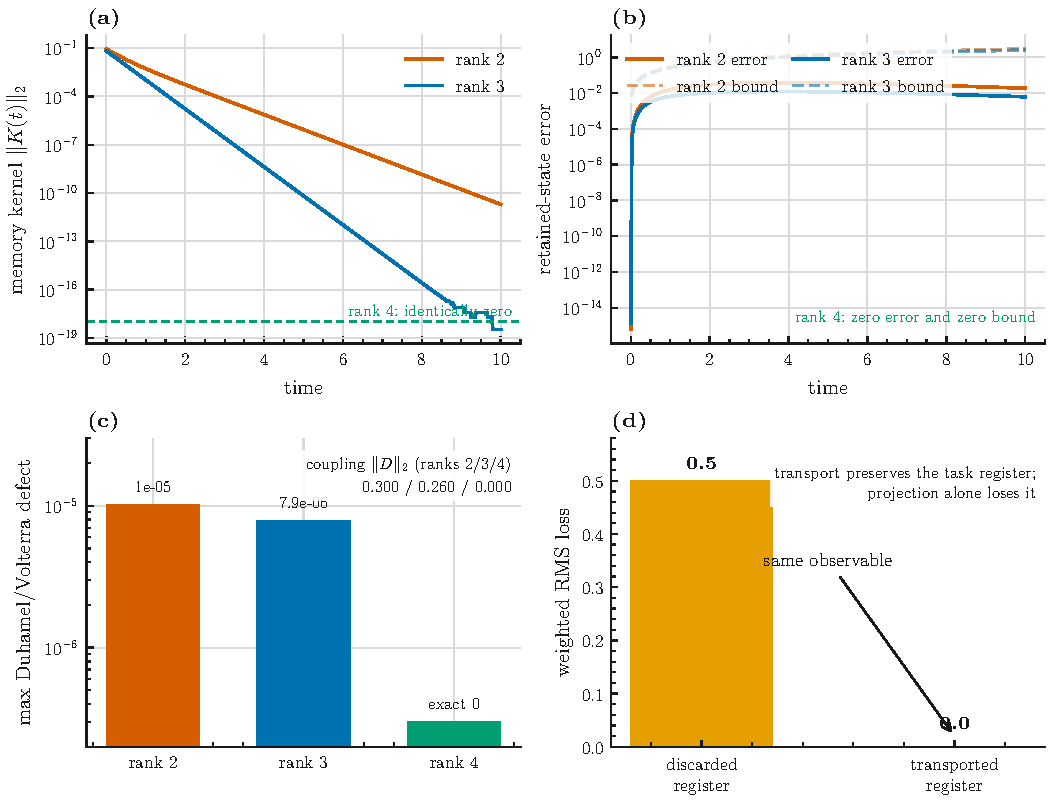
\includegraphics[width=.9\textwidth]{../../../extension/figures/controlled_effective_dynamics_v1.pdf}
\caption{Saved four-state illustration with the generator and retained spaces specified above.
(a) Kernel norm for ranks two and three, with rank four identically zero.
(b) Operator error from omitting memory, bounded by \(t\|B\|_2\).
(c) Residual from trapezoidal evaluation of the exact Volterra equation on the saved grid \(t=0,.025,\ldots,10\).
This quadrature defect is not a model error.
The figure's coupling \(D\) denotes the present \(B\), not the number of categorical fields.
(d) For observable \(f=(0,1,0,1)\), discarding within-group coordinates loses a reference-weighted RMS component \(1/2\), while carrying all internal coordinates gives zero loss.
The example explains which information must accompany group mass when that observable is needed.}
\label{fig:dm-four-state}
\end{figure*}

Positive coarse masses require their own preparation.
Let \(C\) be a \(k\times n\) partition aggregator, with \(C_{\alpha i}=1\) when source state \(i\) belongs to coarse group \(\alpha\).
Let \(\pi_c=C\pi\), assume all groups have positive mass, and define
\begin{equation}
 R=W_\pi C^{\mathsf T}\diag(\pi_c)^{-1},\qquad CR=I_k .
\end{equation}
The column of \(R\) is the reference distribution conditional on that group.
For the preparation \(\rho(0)=R\rho_c(0)\), the coarse propagator
\(T_c(t)=Ce^{tG}R\) is stochastic.
It need not satisfy a semigroup law:
\begin{equation}
 T_c(t+u)-T_c(t)T_c(u)
   =Ce^{tG}(I-RC)e^{uG}R .
\end{equation}
A general preparation \(R\rho_c(0)+\eta_{\rm raw}\), with \(C\eta_{\rm raw}=0\), adds \(Ce^{tG}\eta_{\rm raw}\).
Exact lumpability \(CG=G_cC\) is sufficient for closure.

The partition is a special retained subspace.
Specifically,
\(U_C=W_\pi^{1/2}C^{\mathsf T}\diag(\pi_c)^{-1/2}\)
is an isometry.
A general \(U\) may retain extra signed within-group directions.
For a source test \(f\), write \(a=W_\pi^{1/2}f\).
The reconstructed expectation from \(z\) is
\begin{equation}
 \widehat{\langle f\rangle}
     =f^{\mathsf T}\pi+a^{\mathsf T}Uz ,
\end{equation}
whereas the actual expectation is \(f^{\mathsf T}\rho\).
Their error is
\(a^{\mathsf T}(I-UU^{\mathsf T})y\), giving
\begin{equation}
 \left|\langle f\rangle_\rho-\widehat{\langle f\rangle}\right|
 \leq\|(I-UU^{\mathsf T})a\|
              \sqrt{\chi^2(\rho\Vert\pi)} .
\end{equation}
Here \(\chi^2(\rho\Vert\pi)=\sum_i(\rho_i-\pi_i)^2/\pi_i\).
For \(\rho=\pi(\cdot\mid E)\) with \(\pi(E)=b>0\), this factor is \(\sqrt{b^{-1}-1}\).
A residual norm bounds missing expectation, not the omitted original passage.

If a second isometry \(U_2\) acts on all coordinates retained by \(U_1\), the composite is \(U_1U_2\).
Passing only positive coarse masses while discarding the retained internal coordinates does not implement that composition.
The inherited reference and reconstruction maps must also be passed.
This specifies the composition without introducing an undefined hierarchy of grades or decoders.
It is an optional mathematical result, not an implemented language-pipeline stage.

\section{Structured query protocol}
\label{app:dm-timings}
The primary law enumerates all \(2^{D-1}\) assignments of the first \(D-1\) bits, sets the last bit to even parity and uses unit integer weights.
Dimensions are \(D=13,\ldots,19\).
All tuples are distinct.
Query batches contain \(1,32,256,1024\) positive Boolean product tests.
They fix \(r=0,1,2,4,8,D-1,D\) coordinates, with duplicates removed.
Locations are prefix, suffix or evenly spread when applicable, plus none for \(r=0\) and all for \(r=D\).
Values are taken deterministically from supported witness rows.
Thus the tests have positive empirical mass.
For \(r<D-1\), support fraction is \(2^{-r}\), and for \(r=D-1,D\) it is \(1/N\).

The packed direct comparator evaluates bit masks without materialising a query-by-row matrix.
The weighted-unique comparator first aggregates identical codes and weights.
On the primary law both have \(N\) unique rows.
The exact continuation comparator uses the validated primitive integer representation with a fused width capacity of 128.
That number is an implementation capacity, not a theorem bounding continuation width.
Preflight refuses excess width or memory before preparation.

Two warmups precede eleven samples per served method and shape.
Kernel times use CUDA events.
Full-API wall intervals synchronise the device and include the query API boundary.
The plotted per-regime value is its median full-API time.
The main figure aggregates all nontrivial parity regimes at each size and batch count: the line is their median and the shading their minimum-to-maximum range.
The range describes different queries and locations, not a confidence interval.
Support diagnostics collapse batch count, leaving 112 distinct dimension/fixed-count/location regimes.

The saved matrix records a device-memory total of 3,953,721,344 bytes and explicit resident memory/headroom.
A device model identifier is not present in that matrix.
The timings therefore remain specific to its recorded 4 GB CUDA environment.
A hardware-normalised performance comparison is not established here.
First-use compilation, construction and the source/witness bank are outside the warm query boundary and are reported separately.

\begin{figure*}[t]
\centering
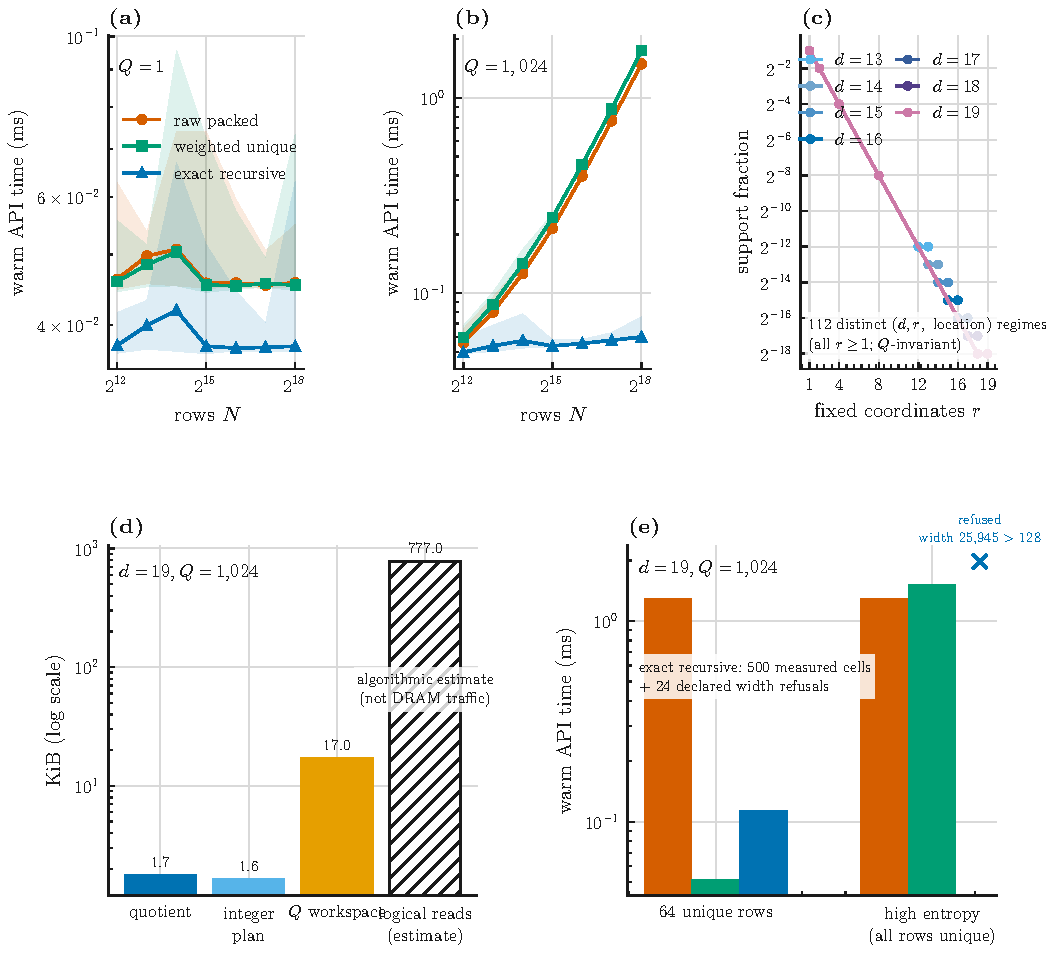
\includegraphics[width=\textwidth,viewport=0 246 504 458,clip]{../../../extension/figures/query_locality_completed_v1.pdf}\\[1ex]
\begin{minipage}[t]{.49\textwidth}\vspace{0pt}\centering
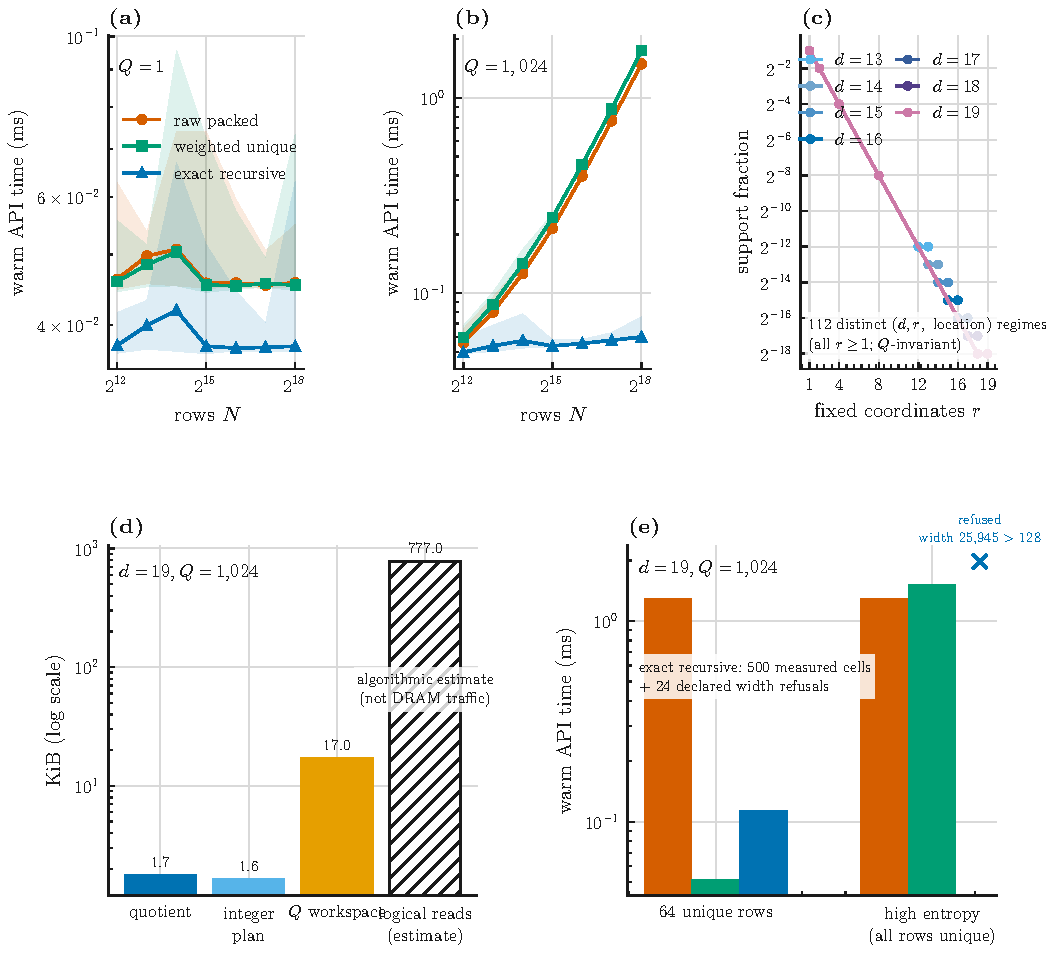
\includegraphics[width=\linewidth,viewport=0 27 247 216,clip]{../../../extension/figures/query_locality_completed_v1.pdf}\\[-.5ex]
{\scriptsize\hspace*{.17\linewidth}\begin{tabular}{cccc}
quotient & integer & query & logical\\
 & plan & workspace & reads (est.)
\end{tabular}}
\end{minipage}\hfill
\begin{minipage}[t]{.49\textwidth}\vspace{0pt}\centering
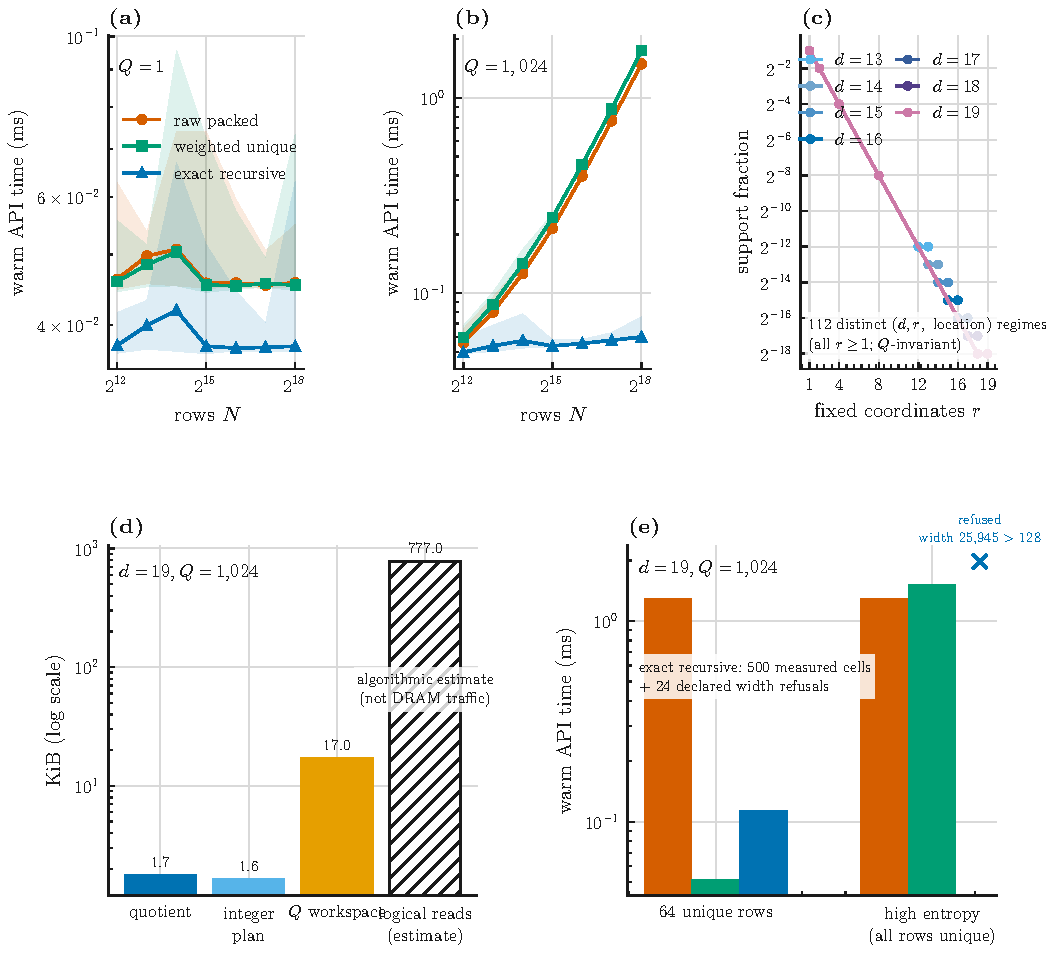
\includegraphics[width=\linewidth,viewport=258 0 504 216,clip]{../../../extension/figures/query_locality_completed_v1.pdf}\\
{\scriptsize Orange: raw packed. Green: weighted unique.\\Blue: exact continuation (cross: width refusal).}
\end{minipage}
\caption{Complete structured-query diagnostic.
(a,b) The parity latency panels used in the main paper.
(c) Query support fraction as the number \(r\) of fixed coordinates changes, for \(D=13,\ldots,19\).
(d) For \(D=19,Q=1024\), quotient storage, integer plan, query workspace and estimated logical reads are different costs.
The last bar is an algorithmic byte-load estimate, not measured DRAM traffic.
(e) Separate control laws, not the parity family: a repeated 64-world support favours weighted direct evaluation, while high-entropy unique support exceeds the continuation kernel's width capacity.
All five original panels are retained as vector crops, with resource labels reset below (d) and an explicit method legend beside (e).
\lq\lq Exact recursive\rq\rq\ in the saved plot means exact continuation evaluation by the integer messages above.
Orange circles denote raw packed scanning, green squares weighted-unique scanning and blue triangles continuation evaluation in (a,b).
The same method colours apply to (e), whose blue cross is a refusal, not a timing.}
\label{fig:dm-all-timings}
\end{figure*}

The secondary laws use a seeded unique half-support of all bit strings, or 64 deterministic unique worlds repeated to the same row count.
They use \(D=13,16,19\), fixed counts four and \(D-1\), and evenly spread locations.
There are 524 recorded cells in all.
Exact continuation executes 500 and agrees with direct integer evaluation.
The remaining 24 are declared width refusals on high-entropy supports.
At \(D=19\), that control has width 25,945 rather than two.
The repeated 64-world support favours the weighted direct method.

At the largest parity size, the weighted-unique control takes \(1739.6\,\mu\mathrm{s}\) per 1024-query batch.
The continuation and integer add-on together use about 3.4 kB, excluding sources, witnesses and query workspace.
Extra construction costs about 55 ms.
Warm precompiled crossover is about 6500 individual single-query calls, or roughly 29,000--41,000 \emph{individual} queries when submitted in batches of 1024.
The latter is of order tens of batch invocations, not tens of thousands of batch invocations.
First-use compilation adds a separate cost.
These are regime-specific amortisation accounts, not a universal speedup.

For an overflow-safe sorting build, comparison and prefix-slot work is bounded by
\(O(DN\log N+\sum_gP_gc_g)\), with \(P_g\) unmerged prefixes.
The compact quotient may be much smaller than that input.
The GPU implementation uses immutable snapshots followed by full construction.
The CPU revision fixture described above is separate.
Its success cannot be combined with these GPU timings into a measured incremental-GPU speedup.

\section{Text methods}
\label{app:dm-text}
The news and FRAMES cohorts were originally drawn by a deterministic stratified rule.
Within each dataset stratum, questions not in the recorded prior-exposure set were sorted by SHA-256 of \texttt{salt|dataset|qid}, using salt \texttt{relational-frontend|draw-order|v1}, and the first quota entries selected.
News uses 43 each of comparison, temporal, inference and null questions, giving 172.
Null questions ask for information the supplied news collection does not establish.
FRAMES uses 38 each of Multiple constraints, Numerical reasoning, Post processing, Tabular reasoning and Temporal reasoning, giving 190.
For a question with several reasoning labels, the loader's rarest-label stratum supplies its allocation.
The originally excluded exposure sets contain 112 news and two FRAMES questions.
Subsequent development inspected these drawn questions and used their failures to develop delivery and reader instructions.
Their initial draw status does not make the present follow-ups untouched confirmation.
The fit/check halves alternate sorted question IDs within each stratum and are preserved as development labels, not restored independence.

LongMem here means the cleaned LongMemEval-S task~\cite{longmem}, not the unrelated LongMem model.
The completed comparison uses the earlier September final-48 manifest, disjoint from the later 188-question draw and the separate 24-question development set.
Its quotas are seven each of single-session user recall, assistant recall, user preference, multi-session integration, temporal reasoning and knowledge update, plus six abstentions.
The manifest records selection salt \texttt{skein-longmemeval-s-cleaned-v1}.
These 48 questions have also been examined during development.
Their dialogue histories supply the observations, while the question date anchors requested elapsed times.

The finite fixture tests update correctness for admitted counts.
The parity study tests structure-dependent query cost.
The news comparison tests evidence assembly under two stated reading operations.
FRAMES tests source delivery and a missing-needs continuation under a fixed answer rubric.
The shared-index LongMem comparison tests the delivered outcomes of its actual index and packing configuration.
It is not a test of a distinct compressed conditional algorithm.
No score is pooled across these purposes or cohorts.

The common news representation contains 609 articles.
Each article is the title followed by its body.
Two-sentence windows have stride one sentence.
Their vector representation is a 384-component BGE-small-en-v1.5 embedding of the text prefixed by title, outlet and publication date.
The imported fp16 encoder produces the stored half-precision rows, which are dotted in float32 for scoring.
Question and facet vectors use its query role.
Cosine compares unit-normalised vectors in this same space.
A document identity names the article, whereas an outlet label can name many articles.
A window retains its character interval in its article.
The matcher can therefore separate article presence from delivery of the required passage.

The deterministic outlet grammar recognises stored outlet names, a leading-\lq the\rq\ alias and the prefix before a vertical bar where present.
It resolves overlapping mentions in favour of the earlier longest match.
Question clauses split at \lq while\rq\ or \lq whereas\rq.
A date following an outlet mention binds locally, otherwise a leading date can be shared.
With no outlet mention, the initial facet is the whole question with no outlet binding.
This is a finite metadata grammar, not a universal natural-language compiler.

The slot compiler uses the same admitted metadata vocabulary as the source index.
Publication-role dates admit the exact day.
Event or unresolved-role dates admit the declared window from that day through six days later.
A month with a year but no day conditions the stored month label.
Missing time or outlet conditions leave that axis unrestricted.
Unknown labels pass unrestricted axes but fail a known-value constraint.
Support membership is the conjunction of allowed metadata labels on the article's retained tuple.
A recognised outlet or fine-day condition with no supported article gives an empty set, not an invented replacement source.
A month mask is formed only for labels present in the stored coarse vocabulary.
If no month label is recognised, that axis stays unrestricted.
Entity, mechanism and polarity are not hard conditions in the compared news route.

Requirements for table reading are produced by the question compiler, not by a model asked for the answer.
It keeps the question's need text for each recognised outlet/date side and its bound slots.
Where a temporal question names several windows, it emits the dated requirements separately.
The requirement compiler returns an ordered obligation list with IDs, need text, source/date/entity slots and cardinality, plus an operator descriptor \(\{\mathrm{kind},\mathrm{over}\}\) and internal frame parameters.
For news, \texttt{comparison\_query} selects \texttt{compare}.
A \texttt{temporal\_query} selects \texttt{change} when it asks about changed or consistent accounts, or lacks ordering words, and otherwise \texttt{order}.
The change frame records whether \lq yes\rq\ means changed or unchanged, while the order frame records before/after and yes/no form.
Inference and null questions both select \texttt{bridge}.
Thus routing does not reveal a null question's reference abstention.
No gold answer or reference evidence enters compilation.

For the Sporting News question below, the temporal-change rule yields \texttt, \texttt{over=[o1,o2]}, with \lq yes\rq\ meaning changed.
The obligations retain the 4 October ticket-report side and 7 October playoff-report side, each bound to Sporting News and its day.
Their metadata supports are the article sets listed below.
The descriptor says which reports the requested operation needs.
In the reported \texttt{table2} condition it does \emph{not} execute a typed change adjudicator or a numerical event comparison.
The reader receives the obligation needs and bound slots, fills one passage-support row per obligation and writes the answer.
All three retrieval methods receive those same requirements.
Typed witness operators and later growth protocols are separate implementations, not additional stages inferred from these scores.

\subsection{One retained source-to-context trace}
The recorded question is:
\begin{quote}\small
Between the Sporting News report on Inter Miami's season ticket prices following Lionel Messi's arrival published on October 4, 2023, and the Sporting News report on Inter Miami's exclusion from the MLS playoffs published on October 7, 2023, was there a change in the team's postseason prospects as reported by the news source?
\end{quote}
Its two outlet/day supports are Sporting News on 4 October and Sporting News on 7 October.
The former includes article \(d203\), \emph{Inter Miami season tickets: Lionel Messi demand causes 2024 prices soar to most expensive in world}, published at 22:12:56 UTC, and \(d41\), \emph{Chicago Fire vs Inter Miami live score, result, updates, highlights from Lionel Messi in MLS match}, at 23:33:00 UTC.
The latter includes \(d88\), \emph{Inter Miami vs FC Cincinnati live score, result, updates, highlights with Lionel Messi's MLS playoffs on line}, published 7 October at 21:30:00 UTC.
These identifiers distinguish articles, not outlets.

The first retained 2000-token facet-conditioned context uses 1989 tokens and has three original article blocks plus an explicitly derived support table.
The support table lists source identities and dates from retained tuples and is marked as derived, not a passage.
The article blocks merge selected spans in original order, with ellipses at gaps.
The ticket-price block states:
\begin{quote}\small
The pricing structure for 2024 represents an enormous increase over the 2023 costs.
\end{quote}
The earlier match block says Messi \lq\lq did not arrive with the team\rq\rq.
The later match block states:
\begin{quote}\small
Eventually, Alvaro Barreal's 78th-minute goal ended any hope that Inter Miami had to complete a stunning playoff charge, and the defeat coupled with CF Montreal's big 4-1 victory over Portland means Inter Miami are officially out of the postseason running.
\end{quote}
The requested comparison needs an earlier postseason assessment as well as later elimination.
The named ticket article and a match-availability statement do not automatically supply that earlier assessment.
The stored diagnostic marks one of three required facts absent from this context.
We present this as a delivery trace, not a newly judged answer or a fabricated successful reconstruction.

The table-reading prompt supplies requirement IDs, need text, bound outlet and bound date.
For each requirement the reader must return the IDs of passages that state it, or an empty list, and at most 25 words recording what they state, or \lq not stated\rq.
It then writes the answer and cited evidence IDs.
This is an explicit reader operation, not a truth value attached by the selector.
Answer-form rules instead require short alternatives, yes/no answers or an insufficient-information response without the table.
The same rule and schema are applied within each comparison.

\subsection{Assembling evidence}
For every route, cosine scores are combined with \(0.5\) times a BM25 keyword score normalised by its maximum over the scored set.
BM25 uses \(k_1=1.2,b=.75\).
The facet-conditioned route ranks within each exact support, retains up to 400 candidates per facet and merges the lists round-robin with duplicate removal.
A short derived support table is admitted only when its standalone token cost is at most one quarter of the evidence budget.
The diversity-ranked route takes 200 whole-corpus candidates and uses MMR relevance coefficient .7.
The local recursive-summary route searches its 1747 stored summaries together with the shared labelled window layer, without MMR.
RAPTOR's distinction between traversal and collapsed retrieval is methodological context~\cite{raptor}.
This local comparator uses the collapsed approach with adapted leaves and packing.
Its summaries are existing abstractive cluster summaries, not empirical conditional states.
The stored hierarchy was built recursively from embedded 100-token leaves using UMAP reduction and Gaussian-mixture memberships, then summarising each cluster and embedding its summary for the next level.
The local implementation uses GPU clustering with declared fixed-seed/update deviations from public RAPTOR.
The summary adapter requests faithful preservation of names, dates, relations and qualifications, caps each summary at 100 tokens and stores it as a distinct parent node.
The reported comparison reuses those summary texts and their BGE vectors, substituting the common labelled-window leaf layer.
It neither regenerates summaries for this test nor makes the generated text an original source witness.

Packing considers ranked spans in order.
It groups them by article, extends them to sentence boundaries, merges touching spans and presents each article's spans in original order.
Articles are ordered by their best admitted piece.
Gaps are marked, not filled with generated text.
Summary nodes remain separate fixed blocks.
The 2000-token allowance counts the canonical JSON serialisation with \texttt{cl100k\_base}, including labels and metadata.
The reader is Claude Sonnet 5.5 at low effort.
The endpoint is normalised exact match from the preserved scorer.
Needed-fact coverage is diagnostic: a reference fact counts only when a mapped occurrence lies inside the union of delivered original spans of its article.
Reference annotations are used for that diagnostic and scoring, not to choose candidate passages.

The banked extraction path stores a proposed statement even when none of its support quotations survives location checking, marking it \texttt{no\_witness}.
Quote matching normalises whitespace and quote characters only, then requires a substring of that input unit.
Unmatched quotations are dropped, not converted into support.
The downstream tuple assembler retains statement status and witness flags beside categorical fields and sparse piece-to-entity, outlet, day/page and document incidence.
It does not thereby certify semantic support for those fields or turn them into the weighted \((A,B)\) fixture.
The compared news route uses hard source/date support and passage ranking, not these statement fields as an entailment gate.

The finite query construction and this text route share explicit source conditions and retained evidence identities.
The news context stage reuses exact supported article sets and ranks original windows within them.
It does not perform a source-edit experiment, propagate the continuous memory kernel, or assign the exact weighted-record demonstration's correctness to language extraction.
The derived support table is distinguished from original text throughout.
The text results measure the delivered evidence and reader response for the stated configuration.

\section{Additional text outcomes}
\label{app:dm-extra-text}
Figure~\ref{fig:dm-news-rules} preserves the common answer-form condition.
It gives 152, 152 and 148 exact matches, with facet-conditioned discordances \(6\)--\(6\) against diversity ranking and \(9\)--\(5\) against local summaries.
The requirement-table condition in the main paper instead gives \(153/145/147\), with \(9\)--\(1\) and \(7\)--\(1\).
The reader operation therefore changes the observed comparison.
Fact-delivery counts remain \(234/211/205\).
The original within-type alternating split has 88 fit and 84 check questions.
Requirement-table exact-match counts are fit \(78/75/77\) and check \(75/70/70\), in facet-conditioned/diversity/local-summary order.
Answer-form rules give fit \(76/77/75\) and check \(76/75/73\).
These original strata describe the same examined cohort and retain their labels without a held-out claim.
They do not isolate the causal effect of the requirement table or establish selector superiority on fresh questions.
\begin{figure*}[t]
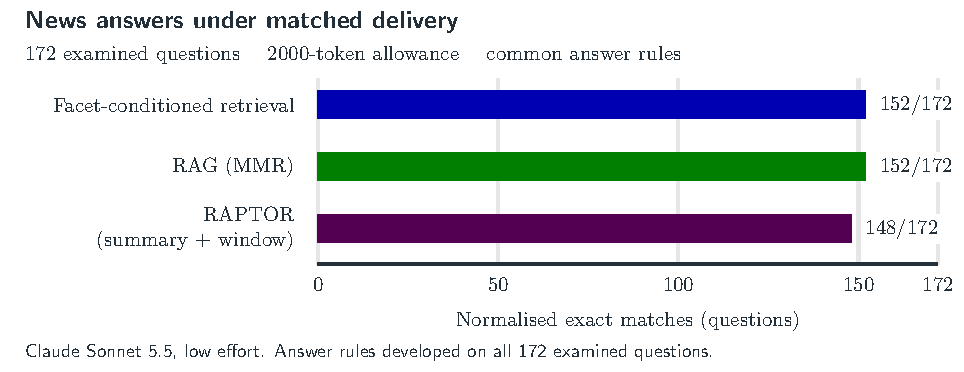
\includegraphics[width=.94\textwidth]{figures/generated/mip_news_matched.pdf}
\caption{Matched-news figure, showing the \emph{answer-form rules} condition.
It is not the requirement-table row in the main paper.
The evidence allowance, labelled windows and local summary adaptation are held fixed within this condition.
\lq\lq RAPTOR\rq\rq\ in this saved figure denotes the adapted local recursive-summary comparator, not a fresh public-system reproduction.
The tie between facet-conditioned and diversity-ranked retrieval is important to the interpretation of the main result.}
\label{fig:dm-news-rules}
\end{figure*}

\begin{table*}[t]
\caption{Additional news method configurations, kept separate from the common-window comparison.
The first row is a different 48-question news cohort, not LongMem, balanced at 12 questions per news type.
The other rows reuse the fixed 100-token-leaf contexts with distinct reader settings.
No score is pooled across rows.}
\begin{ruledtabular}
\begin{tabular}{lrrrr}
Configuration & Questions & Source-conditioned & Flat retrieval & Local summaries\\
\hline
100-token passages, Sol reader &48&40&39&35\\
100-token fixed contexts, Sonnet 5.5 low &172&133&125&118\\
100-token fixed contexts, Sol 5.6 low &172&140&132&130\\
\end{tabular}
\end{ruledtabular}
\end{table*}
In the fixed-context configuration, flat retrieval uses cosine top 40 on 100-token leaves, MMR .7, at most 20 objects and first-fit packing.
The local RAPTOR index has 14,359 leaves and 1747 summaries, takes its cosine top 20 and uses the same local first-fit packing limit.
The allowance is 2000 \texttt{cl100k\_base} tokens.
The stored tree and vectors are reused without a fresh build.
The 48-question configuration also has a flat metadata control with 40 correct answers and byte-identical contexts to the source-conditioned route.
The first row supplies an end-to-end configuration observation on a different draw.
The two 172-question rows hold each method's stored 100-token contexts fixed while changing the reader.
They show sensitivity to reading configuration, not a fresh retrieval gain, a controlled comparison against the common-window route or an isolated effect of the conditional quotient.

\subsection{FRAMES}
FRAMES evaluates retrieval, factual response and reasoning together~\cite{frames}.
The retained source-conditioned comparison uses no entity-activation narrowing beyond its declared source route.
Its initial candidate head comprises fifty pieces ranked by cosine plus .2 normalised BM25.
The implementation recovers page links by exact registered-title mentions in passage text, not by fetching live hyperlinks.
For the selected \texttt{link:mass} route, scores of the top twenty pieces are accumulated on the pages they name.
The five largest target-page totals contribute their best question-scoring piece, followed by the remaining ranked tail.
This is one recovered title-link hop.
Entity-activation witnesses are off in the reported configuration.
Merged sections combine selected spans from the same source section before delivery.

The initial evidence allowance is 8000 tokens, with an instruction to make the necessary reasoning steps explicit.
A missing fact identified by the reader triggers at most one further retrieval and up to 4000 tokens of new spans.
For the diversity control, pass-one relevance is
\(r+.4h/\max h\), with \(r=\mathrm{cosine}+.2\,\mathrm{BM25}/\max\mathrm{BM25}\) and \(h\) the dense seed score.
MMR's relevance coefficient is separately .7 on 200 candidates.
Pass two ranks a missing-need phrase using \(r(\mathrm{phrase})+.5r(\mathrm{question})\), with its own MMR.
Title binding occurs in the \emph{missing-need pass}, not as an oracle mapping the initial question to answer pages.
The title dictionary is built from registered ingested page titles.
The matcher tokenises the reader's need phrase, starts at capitalised or digit-leading tokens, and tries the longest registered sequence of at most eight tokens.
Its last token must also be capitalised or digit-leading.
Matching itself is case-folded.
For example, a phrase naming \emph{Kermanshah Province} aims at that page only if its tokens match a registered title.
It is not a semantic entity resolver.
For each named page, the source-conditioned route prepends its three highest-scoring pieces under \(r(\mathrm{phrase})+.5r(\mathrm{question})\), then appends the global top-200 phrase ranking.
With no recognised title, that global list is the fallback.
Lists from at most six missing phrases are interleaved and deduplicated.
Already delivered intervals are subtracted, residual pieces shorter than 40 characters are discarded, and merged new spans are packed to 4000 tokens.
The reader sees the old blocks followed by these new blocks.
The diversity control instead applies its own MMR to each phrase list.
Allowances and reading instructions match.

The completed outcomes are 127 versus 126 judged correct and 123 versus 117 lexical-proxy successes on 190 questions.
The judged paired discordances are seven wins and six losses.
The judging agent for these completed follow-ups is Claude Sonnet 5.5 at low effort, using the inherited FRAMES rubric, not the earlier P3 judge's Codex model.
It sees the question, benchmark reference answer and prediction, but not the retrieved passages.
A correct answer must give the same final entity, number, date or alternative as the reference, allowing compatible wording, abbreviations, units and reference-tolerated rounding.
Every required part must be present.
A wrong required part, incompatible value or hedging between alternatives is incorrect.
A refusal is abstained and counts as unsuccessful.
Two batch compositions are judged, with a third decision on disagreement and majority as the final verdict.
This measures reference-answer correctness, not independent verification that cited evidence entails it.

The lexical proxy first accepts normalised exact match.
Otherwise it rejects missing, empty or explicit insufficient-information predictions and any prediction longer than three times the reference's normalised word count.
Normalisation lowercases, removes punctuation and the articles \lq a\rq, \lq an\rq\ and \lq the\rq, then collapses whitespace.
Let \(p\) be the normalised prediction, \(g\) the full reference and \(g_0\) its text before the first full stop or comma, normalised in the same way.
The proxy accepts \(p\subseteq g\), or nonempty \(g_0\) with \(g_0\subseteq p\) or \(p\subseteq g_0\), where \(\subseteq\) here means contiguous substring.
It also accepts token F1 at least .5, using the preserved scorer's token overlap.
This answer-form rule is not semantic correctness.
Figure~\ref{fig:dm-frames} preserves both instead of treating them as the same accuracy measure.
A simpler delivery configuration gives 62/58 judged successes, and an 8k explicit-step configuration before the extra pass gives 106/106.
The large delivery recovery coexists with a small final matched difference.
\begin{figure*}[t]
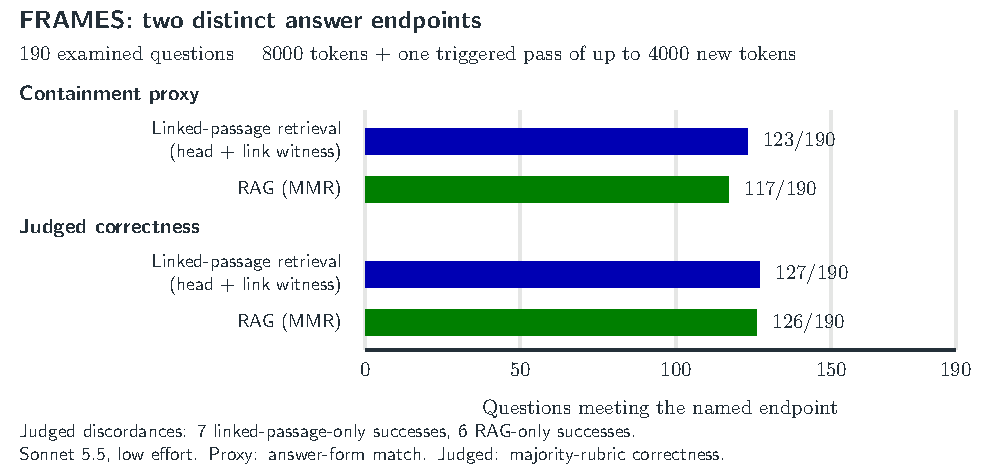
\includegraphics[width=.94\textwidth]{figures/generated/mip_frames_noactivation.pdf}
\caption{FRAMES endpoint comparison.
Lexical-proxy success and judged correctness answer different questions.
Both retrieval routes have the same 8k initial allowance and at most one missing-needs-triggered 4k delivery.
The final judged difference is one answer on 190 questions, not evidence that the methods are equivalent.}
\label{fig:dm-frames}
\end{figure*}

A page in the source bank may omit the required table.
Then page availability is not availability of the needed row.
Other cases deliver relevant facts but require an arithmetic or date operation that the reader fails to complete.
Source availability, located passage support and final correctness identify different points of failure.
Only the completed comparison above is included as an answer outcome.

\subsection{LongMem}
The completed shared-index LongMem comparison retains whole dialogue turns.
Its stored labels \texttt{ours\_keys} (also called relational) and \texttt{dense\_keys} both invoke \texttt{CaseState.dense\_scores("dn",2)}.
There is no distinct compressed conditional reconstruction in this executed arm.
The key \texttt{dn} concatenates the role-labelled raw turn, session date and deterministic normalisations of date mentions and word-form quantities.
Relative expressions are anchored to the turn's session date.
Stored vectors are 384-component BGE-small-en-v1.5 fp16 embeddings, converted to float32 and unit-normalised on loading from the role/text-hashed cache.

For each question-side obligation facet, \texttt{dense\_scores} takes its vector dot product with every turn key.
It then takes a per-turn maximum over the key score, long-turn windows of at most 400 encoder tokens and, with \texttt{views=2}, sentence views of user turns.
Facet-specific stable orders are interleaved round-robin with duplicate removal.
Both arms use these identical facet lists, ties and defaults.
The completed final-48 route has no branch-activation table, no fact ledger and no event-pair operator.
The common packer adds a whole turn when its text tokens plus a twelve-token header allowance fit, skips turns that do not fit, stops below 30 remaining tokens and admits at most 120 turns.
Selected turns are displayed in session-date and within-session order.
Identical question/date/context prompts deliberately share a cached reader response.
Equal predictions here follow equal computation, not an independently measured representation advantage.
The hybrid arm changes the score to .7 times dense plus .3 normalised BM25 before the same facet ordering and packer.

For example, the charity question below asks for two dated events jointly.
The shared-dense score call ranks individual turns, not candidate event pairs.
It has no step that can make both operands obligatory before packing.
This configuration differs from the general exact identities in Eqs.~\eqref{eq:querymass}--\eqref{eq:adjoint} and from the older 32-development-facet transport tests with local vector frames.
Neither is an operation executed by these completed LongMem arms.
The existing figure's \lq\lq Relational retrieval\rq\rq\ label denotes \texttt{ours\_keys}, here a second label for shared-dense execution, not a third reconstruction method.

Correctness includes 48 questions and all six abstentions.
Complete positive evidence uses 42 questions, excluding the six.
Conditional and dense readouts give \(44/48\) and \(45/48\) correct at 4k and 8k, with \(41/42\) positive-evidence coverage at both allowances.
Hybrid gives \(40/48,44/48\) correct and \(33/42,37/42\) positive coverage.
A separate nonempty-annotation endpoint has denominator 44 because two abstention questions also have annotated required turns.
Its preserved counts are \(43/44\) for conditional and dense, and \(35/44,39/44\) for hybrid.
The denominators measure different populations rather than replacing one another.
\begin{figure*}[!htbp]
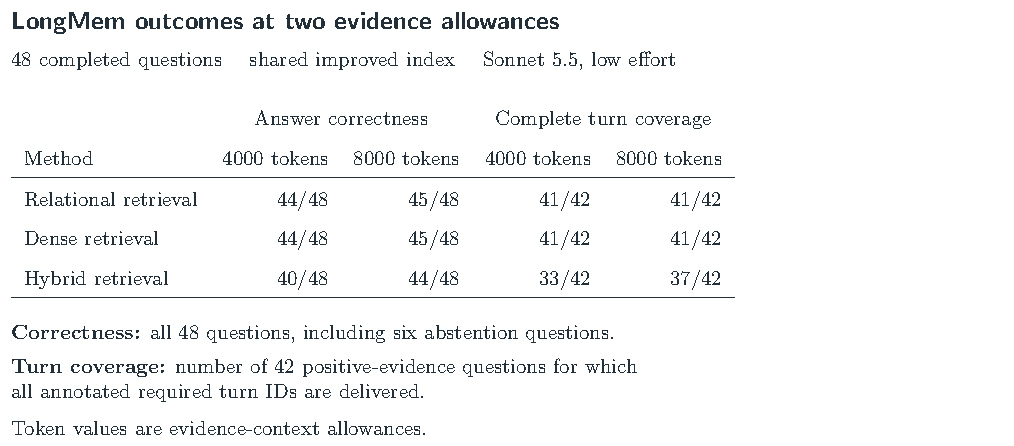
\includegraphics[width=.94\textwidth]{figures/generated/mip_longmem_completed.pdf}
\caption{Completed shared-index LongMem comparison.
Answer correctness includes all 48 questions and six abstentions.
Complete required-turn coverage uses 42 positive-evidence questions.
The saved \lq\lq Relational retrieval\rq\rq\ and dense series are the shared-dense \texttt{ours\_keys} and \texttt{dense\_keys} arms defined above.
They invoke the same score call and packer, not different exact readout implementations.
Evidence-context allowances are 4000 and 8000 tokens.}
\label{fig:dm-longmem}
\end{figure*}

The unresolved positive case asks for elapsed months since two charity events on consecutive days.
Required primary turn ranks are 73, 88, 100, 116 and 134.
The 4k and 8k packs stop after ranks 27 and 54.
The missing primary turns are eligible but not reached before packing stops.
A delivered paraphrase overlaps one event, so primary-ID coverage is not a complete measure of semantic availability.
The decisive pair is not jointly delivered by the executed route.
Hybrid can supply it at 8k but has lower aggregate positive coverage.
This identifies a candidate temporal composition operation to test, not a demonstrated benefit of budget alone.

\par

\clearpage
\bibliography{reconstruction_refs}
\end{document}
